%--------------A VOTRE ATTENTION-------------%
% Les étudiants en master qui disposent de plus de 3 chapitres dans leurs travaux peuvent en complèter
% Les Membres doivent figurer dans la dernière version finale du mémoire après soutenance pour dépôt de mémoire

\documentclass{ifri}
\usepackage{titletoc}

%\usepackage[utf8]{inputenc}   %gestion des accents
\usepackage[T1]{fontenc} %gestion des accents
\usepackage{eurosym}
\usepackage{listings}
\usepackage{xcolor}
\usepackage{graphicx} %LaTeX package to import graphics
\graphicspath{{images/}} %configuring the graphicx package
%\usepackage[francais]{babel} %pour accent apostrophe
\definecolor{codegreen}{rgb}{0,0.6,0}
\definecolor{codegray}{rgb}{0.5,0.5,0.5}
\definecolor{codepurple}{rgb}{0.58,0,0.82}
\definecolor{backcolour}{rgb}{0.95,0.95,0.92}
\lstdefinestyle{mystyle}{
    backgroundcolor=\color{backcolour},   
    commentstyle=\color{codegreen},
    keywordstyle=\color{magenta},
    numberstyle=\tiny\color{codegray},
    stringstyle=\color{codepurple},
    basicstyle=\ttfamily\footnotesize,
    breakatwhitespace=false,         
    breaklines=true,                 
    captionpos=b,                    
    keepspaces=true,                 
    numbers=left,                    
    numbersep=5pt,                  
    showspaces=false,                
    showstringspaces=false,
    showtabs=false,                  
    tabsize=2
}

\usepackage{caption}
\newcommand{\source}[1]{\caption*{Source: {#1}} }


\newcommand*{\captionsource}[2]{%
  \caption[{#1}]{%
    #1%
    \\\hspace{\linewidth}%
    \textbf{Source:} #2%
  }%
}

\lstset{style=mystyle}
%\usepackage[T2A]{fontenc}
%\usepackage[utf8]{inputenc}

\setlength{\glsdescwidth}{0.65\textwidth}
% \usepackage{lscape}

\typeMemoire{Diplôme de Master en Informatique}
\optionFormation{Systèmes d'Information et Réseaux Informatiques}
\etudiant{Sero Abdel-Kader \textbf{SAKA}}
\titreDuMemoire{Mise en place d'un Cloud Rest API pour l'identification et l'authentification de locuteur par empreinte vocale}

\dateSoutenance{- Fevrier 2023}
%\promo{2\up{ème}}
\anneeScolaire{2019-2021}


%%maitre de mémoire
\encadrants{Dr John \textbf{AOGA} }


%% Membres du Jury
\jurys{%
\begin{tabular}{llll}
	Nom et prénoms du président & Grade & Entité & Président \\
	Nom et prénoms de l'examinateur & Grade & Entité & Examinateur \\
	Nom et prénoms du rapporteur & Grade & Entité & Rapporteur \\
\end{tabular}	
}


\hypersetup{
 pdftitle={--},
 pdfauthor={--},
 pdfsubject={--},
 pdfkeywords={--} 
 }

\color{bookColor}

%importation du glossaire
\loadglsentries{glossaire_reduit}

\begin{document}

\pageDeGarde
%\pageTitre

\pagecolor{white}

%% page vide
%\thispagestyle{empty}\ \clearpage


\selectlanguage{french}

% sommaire
\pagenumbering{roman}

\setcounter{tocdepth}{0}
\startlist{toc}
\printlist{toc}{}{\chapter*{Sommaire}}
\setcounter{tocdepth}{5}

%% rdedicaces
\dedicace
Je tiens à dédier ce travail à la
mémoire de mon père disparu trop tôt. J’espère que,
du monde qui est sien maintenant, il apprécie cet
humble geste comme preuve de reconnaissance de la
part d’un fils qui a toujours prié pour le salut de son
âme. Puisse Dieu, le tout puissant, l’avoir en sa
sainte miséricorde ! 



\newpage 

%% remerciements
\remerciements

C’est avec un grand plaisir que je réserve ces quelques lignes en signe de gratitude et de
profonde reconnaissance à tous ceux qui, de près ou de loin, ont contribué à la réalisation et
l’aboutissement de ce travail.\\Je tiens tout d’abord à remercier Le \textbf{Docteur John AOGA} pour son soutien, son accompagnement, et surtout pour son aide précieuse tout au long de l’élaboration de ce travail.\\Notre parfaite gratitude au corps professoral de l’\textbf{ IFRI }en général et plus particulierement au \textbf{Prof. Eugène C. EZIN, Directeur de l’Institut de Formation et de Recherche en Informatique (IFRI)}.\\Je m’acquitte, enfin, volontiers d’un devoir de gratitude et de remerciements à \textbf{tous mes
enseignants} pour la qualité de l’enseignement qu’ils ont bien voulu me prodiguer durant mes études afin de me fournir une formation efficiente. 
\newpage 

% Résume
\resume
\selectlanguage{french}
\vspace*{-6cm}
\begin{abstract}
    \paragraph{}La parole est le moyen principal et le plus pratique de communication entre les gens. Que ce soit par curiosité technologique de construire des machines qui imitent les humains ou par le désir d'automatiser le travail avec des machines, la recherche en reconnaissance de la parole et des locuteurs, comme première étape vers une communication naturelle homme-machine, a suscité beaucoup d'enthousiasme au cours des cinq dernières décennies. 
    \paragraph{}La reconnaissance de locuteur (RL) est le processus d'identification d'un locuteur en fonction des caractéristiques vocales de la parole donnée. Cela diffère de la reconnaissance de la parole où le processus d'identification est limité au contenu plutôt qu'au locuteur. Le processus de SR repose sur l'identification et l'extraction des caractéristiques uniques de la parole du locuteur. Les caractéristiques de la voix de la personne sont également connues sous le nom de biométrie vocale.
    \paragraph{}Un système de Reconnaissance de Locuteur (RL) est utilisé pour identifier et distinguer les locuteurs et extraire des caractéristiques uniques qui peuvent être utilisées pour la vérification ou l'authentification de l'utilisateur. L'identification de locuteur (IL) est connue comme le processus d'identification du locuteur à partir d'une énonciation donnée en comparant la biométrie vocale de l'échantillon donné du locuteur. Lorsque la voix est utilisée pour l'autorisation, on parle de vérification du locuteur. Le domaine d'application clé de la RL est la sécurité et les sciences médico-légales. 
    \paragraph{}Les systèmes de RL sont également utilisés comme remplacement des mots de passe et d'autres processus d'authentification des utilisateurs (mot de passe vocal). Les sciences médico-légales appliquent la RL pour comparer les échantillons vocaux de la personne prétendument impliquée avec d'autres preuves obtenues, telles que des conversations téléphoniques ou d'autres preuves enregistrées. Ce processus est également appelé détection de locuteur. 
    \paragraph{}L'aspect le plus important de l'utilisation des systèmes d'IL est l'automatisation de processus tels que la redirection des courriers des clients vers la bonne boîte aux lettres, la reconnaissance des interlocuteurs dans une discussion, l'avertissement des systèmes de reconnaissance de discours en cas de changements de locuteur, la vérification si un client est enregistré dans le système, etc. Ces systèmes d'IL peuvent fonctionner sans la connaissance de l'échantillon vocal d'un client car ils se fient uniquement à l'identification d'un locuteur d'entrée à partir de la base de données existante de locuteurs.
    \paragraph{}Par conséquent, l'objectif de cette étude est de réaliser une revue systématique de la littérature sur les diverses approches de reconnaissance de locuteur et d’implémenter l’approche la plus prometteuse.

\paragraph{}
\textbf{Mots clés}: Reconnaissance de la parole et des locuteurs, biométrie vocale, échantillon vocal, biométrie vocale, reconnaissance de la parole
    
\end{abstract}

\newpage
\thispagestyle{empty}
\selectlanguage{english}
\addcontentsline{toc}{chapter}{Abstract}
\begin{abstract}

\paragraph{}Speech is the primary, and the most convenient means of communication between people. Whether due to technological curiosity to build machines that mimic humans or desire to automate work with machines, research in speech and speaker recognition, as a first step toward natural humanmachine communication, has attracted much enthusiasm over the past five decades.
\paragraph{}Speaker Recognition (SR) is the process of identifying the speaker according to the vocal features of the given speech. This is different to speech recognition where the identification process is confined to the content rather than speaker. The process of SR is based on identifying and extracting unique characteristics of the speaker's speech. The characteristics of voices of the person is also known as voice biometrics.
\paragraph{}A SR system is used to identify and distinguish speakers and extract unique characteristics that may be used for user verification or authentication. Speaker Identification (SI) is known as the process of identifying the speaker from a given utterance by comparing voice biometrics of the given sample of the speaker. 
\paragraph{}When voice is used for authorization, it is termed as Speaker Verification. The key application area of SR is security and forensic science. SR systems are also used as a replacement for password and other user authentication processes (voiced password). Forensic science applies SR to compare the voice samples of the person claimed to be with other evidences obtained like telephone conversation or other recorded evidence. 
\paragraph{}This process is also referred as speaker detection. The most important aspect of using SI systems is for automating processes like directing clients’ mails to the right mailbox, recognizing talkers in discussion, cautioning discourse acknowledgment frameworks of speaker changes, checking if a client is enlisted in the framework as of, and so on. These SI systems may work without the knowledge of a client's voice sample since they rely only on identifying an input speaker from the existing database of speakers.
\paragraph{}Therefore, the objective of this study is to conduct a systematic literature review on various speaker recognition approaches and implement the most promising approach.


\paragraph{}
\textbf{Key words}: research in speech and speaker recognition, Speaker Recognition (SR), speech recognition, voice biometrics, voice sample
\end{abstract}
\newpage

%liste des figures
\listoffigures 
\newpage

%liste des tableaux
% \listoftables
% \newpage

%liste des algo
\selectlanguage{french}
\listofalgorithmes
\newpage

% Les sigles et acronymes
\setglossarystyle{altlist}
\printglossary[title=Liste des acronymes, toctitle=Liste des acronymes, type=\acronymtype]
\newpage

% Le glossaire proprement dit
%\setglossarystyle{super}
%\printglossary[type=main]


\pagenumbering{arabic}
\setcounter{page}{1}
%%introduction
\introduction
%\paragraph{}bla bla bla \gls{acro} puis \Gls{acroglo} et enfin \gls{glossaire}

%1-	Problématique
\paragraph{}Les temps ont changé, l’heure est à la mobilité. Or les usages et les règles de sécurité qui fonctionnaient à domicile sur un PC sont plus difficilement applicables en situation de mobilité, où l’usage du mot de passe atteint ses limites. Et pourtant, plus que jamais, il est primordial de protéger nos contenus, nos transactions et notre identité.
\paragraph{}La problématique de l'authentification par mot de passe ou code pin est liée à la sécurité des données et à la facilité d'utilisation. En effet, d'un côté, l'utilisation d'un mot de passe ou d'un code pin peut garantir la confidentialité des informations personnelles et des données sensibles, en empêchant l'accès aux tiers non autorisés. D'un autre côté, ces méthodes d'authentification peuvent être facilement compromises, par exemple, en utilisant des attaques de force brute ou de phishing, ou en découvrant le mot de passe ou le code pin par l'observation ou la divulgation.
\paragraph{}De plus, la complexité et la longueur des mots de passe peuvent rendre leur utilisation difficile et fastidieuse pour les utilisateurs, tandis que les codes pin peuvent être plus faciles à retenir mais également plus faciles à deviner.
\paragraph{}Ainsi, la question de l'authentification par mot de passe ou code pin est un compromis entre la sécurité et la convivialité, et doit être abordée avec prudence et en prenant en compte les risques potentiels et les besoins des utilisateurs. 
\paragraph{}La reconnaissance par biométrie vocale est une technologie qui utilise la voix comme moyen d'authentification et de reconnaissance d'identité. Elle peut être utilisée dans de nombreux domaines tels que la sécurité, l'accès à des services en ligne, la surveillance ou encore la gestion des appels téléphoniques. Cependant, cette technologie soulève des problématiques importantes en termes de protection de la vie privée, de fiabilité des systèmes et d'éthique. De plus, les données vocales collectées peuvent être utilisées à des fins malveillantes si elles tombent entre de mauvaises mains. Enfin, la biométrie vocale pose des questions quant à la protection de la vie privée et des libertés individuelles, notamment en ce qui concerne l'utilisation des données vocales pour la surveillance de masse ou la reconnaissance automatique de la voix dans les médias.
\paragraph{}Comment garantir la sécurité et la confidentialité des données collectées ? Comment éviter les erreurs de reconnaissance et les usurpations d'identité ? Quelles sont les conséquences éthiques de l'utilisation de la biométrie vocale ? Autant de questions auxquelles il est nécessaire de répondre pour assurer une utilisation responsable et efficace de cette technologie. 


%2-	Contexte et justif
\paragraph{}Face à la fraude documentaire et au vol d'identité, aux menaces du terrorisme ou de la cybercriminalité, et face à l'évolution logique des réglementations internationales, de nouvelles solutions technologiques sont progressivement mises en œuvre.
\paragraph{}Parmi ces technologies, la biométrie s'est rapidement distinguée comme la plus pertinente pour identifier et authentifier les personnes de manière fiable et rapide, en fonction de caractéristiques biologiques uniques.
\paragraph{}Aujourd'hui, de nombreuses applications font appel à cette technologie.
\paragraph{}Ce qui était autrefois réservé à des applications sensibles telles que la sécurisation de sites militaires est devenue une application grand public en développement rapide.
\paragraph{}Un simple geste de la main, une pression du doigt sur un capteur, une expression prononcée de la voix, ou un regard d’une seconde vers une caméra suffisent pour prouver son identité.
\paragraph{}L’authentification biométrique vocale facilite la vie des consommateurs et citoyens qui sont de plus en plus mobiles et connectés en leur apportant une alternative simple aux mots de passe et aux codes PIN pour s’authentifier. 
\paragraph{}Ainsi nous souhaiterons mettre en place un Cloud API pour l’authentification et l’identification des individus par biométrie vocale.

%3-	Objectifs
\paragraph{}L’objectif principal de notre étude est de concevoir déveloper et déployer un Cloud AI pouvant être appelé par REST API capable d’authentifier et d’identifier les individus à travers leur biometrie vocale. La matérialisation de cet objectif, passera par l’aboutissement des objectifs spécifiques que sont: 

\paragraph{}De façon spécifique, il s’agira :
\begin{itemize}
    \item la mise  en place la sauvegarde et l’organisation du dataset; 
    \item le choix des outils, des technologies  et de architecture à adopter ; 
    \item la mise en place de modèles d'IA  permettant les operations d’identification et d’authentification par biometrie vocale ; 
    \item la création mise en place des REST APIs;
\end{itemize}

%4-	 Organisation du mémoire
\paragraph{}Outre l’introduction et la conclusion, le present memoire comprend quatre (04) chapitres.
\paragraph{}Le premier chapitre présente l’état de l’art de l’identification par biometrie vocale.  Dans le deuxième chapitre nous explorons les materiels et méthodes. Le troisième chapitre nous permet d’exposer la modelisation et le developpement de notre model d’IA. Le quatrième chapitre nous permet de présenter les resultats découlant de nos travaux. Nous faisons ensuite une discussion et présentons les difficultés rencontreées dans la réalisation de  cette étude. 

%\lhead[]{} \rhead[]{} \chead[]{}
\selectlanguage{french}
\fancyhead[L]{\tiny \leftmark}
\fancyhead[R]{\scriptsize \rightmark}
\fancyfoot[C]{\thepage}

\chapter{ETAT DE L’ART DE IDENTIFICATION PAR BIOMETRIE VOCALE}\label{chap:1}
 \addcontentsline{toc}{section}{Introduction}
\section*{Introduction}
L’identification par biométrie vocale est le processus de reconnaissance et de vérification de l’identité d’une personne à partir de leur enregistrement vocal. Elle a des applications importantes telles que la sécurité a criminalistique, l’IoT, les centres d’appel, et l’interaction homme-machine. Elle a été révolutionnée par les techniques d’apprentissage profond ces dernières années, permettant une identification plus précise, même dans des environnements acoustiques difficiles avec des parasites sonores. Ces techniques exploitent de grandes quantités de données vocales pour former des modèles de réseaux neuronaux qui peuvent apprendre à extraire automatiquement des caractéristiques discriminantes des signaux vocaux.

Dans ce chapitre, nous clarifierons d’abord les concepts clés liés à notre étude. Par la suite nous présenterons les quelques techniques de mise en place de ce type de modèles d’Intelligence Artificielle.

\section{Définitions}
\subsection{Biométrie}

La biométrie comprend tout un ensemble de technologies et procédés de reconnaissance, d’authentification et d’identification des personnes à partir de certaines de leurs caractéristiques physiques (empreintes digitales, la forme de la main, du doigt, le réseau veineux, l'œil), biologiques (ADN, le sang, la salive) ou comportementales (reconnaissance vocale, la dynamique des signatures). Ces caractéristiques doivent être à la fois \cite{idemia} :	
\begin{itemize}
    \item Universelles : pour être utilisables par tous ; 
    \item Uniques : pour distinguer les personnes sans équivoque;
    \item Invariables : pour permettre une utilisation tout au long de la vie;
    \item Mesurables : pour permettre la comparaison.
\end{itemize}

Les différentes techniques utilisées font l'objet de recherches régulières, de développements et bien entendu, d'améliorations constantes.
Toutefois, les différentes sortes de mesures n'ont pas le même niveau de fiabilité.
On estime que les mesures physiologiques ont l'avantage d'être plus stables dans la vie d'un individu.
Par exemple, elles ne subissent pas autant les effets du stress, contrairement à l'identification par mesure comportementale \cite{idemia}.

\subsection{Biométrie vocale}
l'authentification par Biométrie vocale consiste à utiliser la voix d'une personne comme caractéristique biologique d'identification unique afin de l'authentifier.
La Biométrie vocale est considérée comme la méthode d'authentification la plus solide car elle lie l'identité à un individu réel \textbf{("ce que vous êtes" plutôt que "ce que vous savez" ou "ce que vous avez")}.
Elle  extrait un ensemble de caractéristiques audio qui garantissent qu'un locuteur est une personne réelle plutôt qu'un enregistrement ou un synthétique voix d'un individu \cite{nice}.
%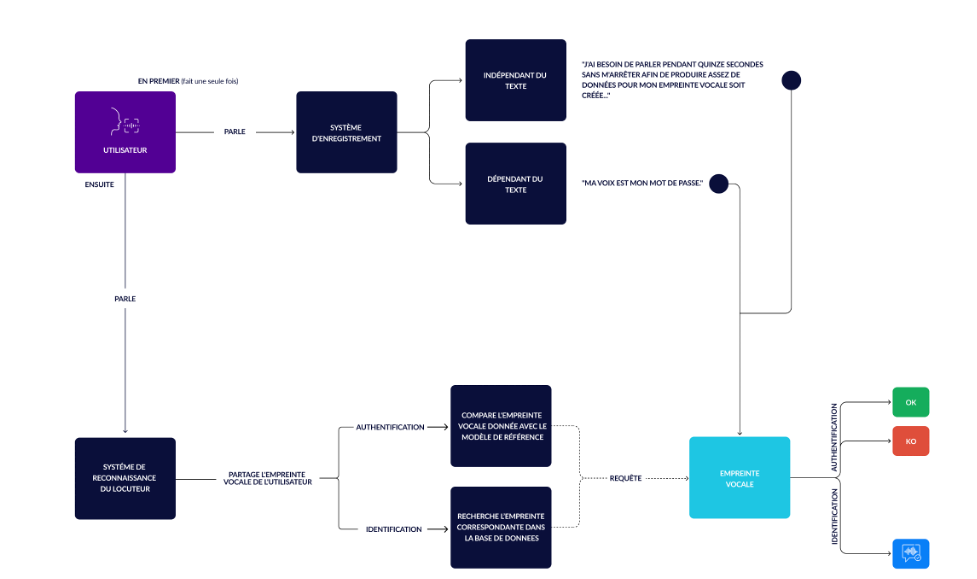
\includegraphics{1-Picture1}  
%1-Picture1.png
\begin{figure}[ht]
    \centering
    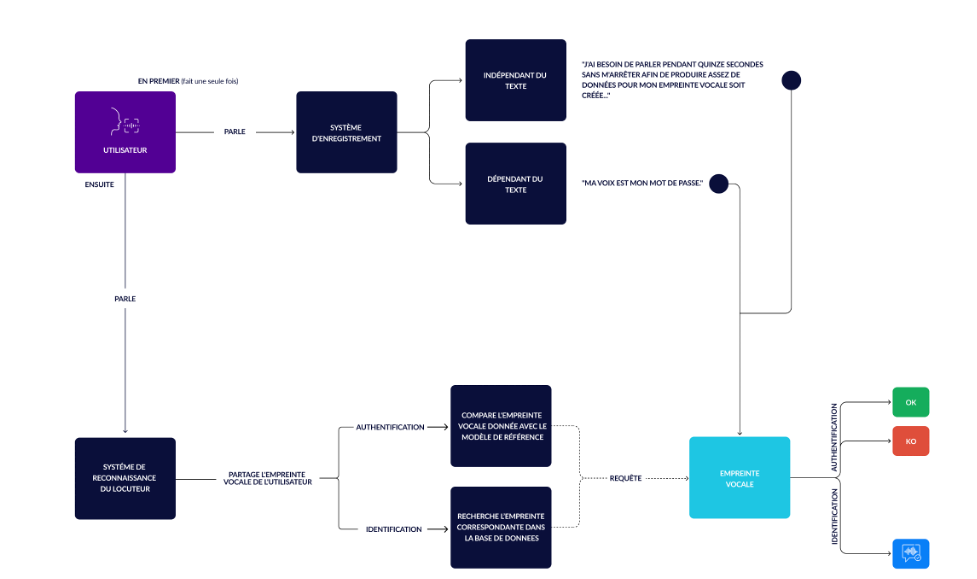
\includegraphics[width=1\textwidth]{1-Picture1}
    \caption{Architecture d'une IA de reconnaissance par biométrie vocale.}
    \label{fig:1-Picture1}
    \source{Source of the image.}
\end{figure}

\subsection{Identification et authentification biométrique}
La biométrie permet l'identification et l'authentification d'une personne à partir de données reconnaissables et vérifiables, qui lui sont propres et qui sont uniques.
\paragraph{}\textbf{L'identification }consiste à déterminer l'identité d'une personne.
Il s'agit de saisir une donnée biométrique de cette personne, en prenant par exemple une photo de son visage, en enregistrant sa voix, ou en captant l'image de son empreinte digitale. Ces données sont ensuite comparées aux données biométriques de plusieurs autres personnes qui figurent dans une base; \textbf{ ici, on essaye de répondre à la question: « qui êtes-vous ? »}.
\paragraph{}\textbf{L'authentification}, appelée également vérification, est le processus qui consiste à comparer les données caractéristiques provenant d'une personne, au modèle de référence biométrique de cette dernière (« template »), afin de déterminer la ressemblance. Le modèle de référence est préalablement enregistré et stocké dans une base de données, dans un équipement ou objet personnel sécurisé. On vérifie ici que la personne présentée est bien la personne qu'elle prétend être.
Dans ce cas on essaye de répondre à la question: « êtes-vous bien celui que vous prétendez être ? ».
\subsection {Deep learning}
\textbf{Le deep learning ou apprentissage profond}  est une technique d'apprentissage automatique basée sur des réseaux de neurones artificiels. Dans le domaine de la reconnaissance vocale, l'apprentissage profond est largement utilisé pour améliorer la précision de la reconnaissance \cite{embeddings}.


\section{historique de la biométrie vocale}
La biométrie répond à une préoccupation très ancienne de prouver son identité, de manière irréfutable, et en utilisant nos différences et particularités.
\paragraph{}\textbf{1952}: le premier système de reconnaissance vocale a été développé par Lawrence G. Roberts et ses collègues au laboratoire Lincoln du MIT. Le système utilisait l’analyse spectrographique de fichiers vocaux comparé á une base de données de d’empreintes vocales de personnes bien identifiées.
\paragraph{}\textbf{1962}: les laboratoires Bell ont créé le système "voiceprint", qui utilise un spectrogramme pour analyser les modèles de fréquence uniques de la voix d’un locuteur afin de les identifier. 
\paragraph{}\textbf{Années 1970}: Plusieurs systèmes d’identification de d’individus par empreinte vocale commerciaux ont été développés, y compris le système VeriVox de Raytheon et le système VoiceID de Bolt Beranek et Newman (BBN).
\paragraph{}\textbf{Années 1990}: Les chercheurs ont commencé à explorer l’utilisation de réseaux neuronaux pour l’identification des individus par voix, ce qui a permis une identification plus précise et plus fiable.
\paragraph{}\textbf{Années 2000}: L’identification des individus par voix est devenue plus largement utilisée dans les applications d’application de la loi et de sécurité, et les chercheurs ont commencé à explorer l’utilisation d’algorithmes d’apprentissage automatique pour identifier automatiquement les locuteurs sans avoir besoin d’une base de données préexistante de locuteurs connus. 
\paragraph{}Aujourd’hui, l’identification des individus par voix continue d’être un domaine de recherche actif, avec des applications dans divers domaines, notamment l’application de la loi, la sécurité et la criminalistique.


\section{Types de reconnaissances vocales}
Les principes de la biométrie vocale sont généralement séparés en 2 types :
\begin{itemize}
    \item Dépendant du texte : \\Ce type de reconnaissance du locuteur exige que l’utilisateur dise exactement l’expression enregistré. Cela manque de flexibilité étant donné que l’utilisateur doit se souvenir de ladite expression, mais offre une précision et une rapidité intéressantes.
    \item Independant du texte : \\Ce processus de vérification n’a pas la contrainte de contenu. L’utilisateur peut parler librement. Toutefois, l’entraînement et les tests d’énonciation prendront plus de temps pour atteindre la performance attendue \cite{timedoctor}.
\end{itemize}

\section{Fonctionnement}
La Biométrie vocale utilise des modèles de voix pour générer une identification unique pour chaque individu, en travaillant avec plus de 100 caractéristiques physiques et comportementales. Il comprend la vitesse de la parole, l'accent, la prononciation, l'emphase, en plus des facteurs physiques de vos voies vocales, de votre bouche et de vos voies nasales \cite{imageware}.

\begin{figure}[h]
    \centering
    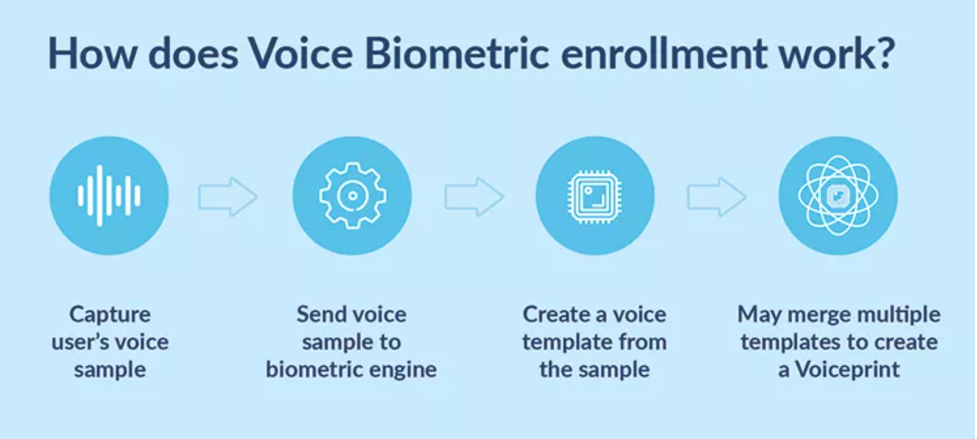
\includegraphics[width=1\textwidth]{2-fonctionnement}
    \caption{Ajout d'un individu à une IA de reconnaissance parempreinte vocale.}
    \label{fig:2-fonctionnement}
\end{figure}

Selon la méthode d’authentification (dépendante du texte ou indépendante du texte), une IA de biométrie vocale collecte le modèle vocal d’un utilisateur \cite{rcdevs}. Cependant, il n’authentifie pas ce que l’utilisateur dit. Il vérifie seulement qui parle.
Il extrait les caractéristiques qui distinguent le discours d’une personne des autres. Le résultat est une empreinte vocale ou un modèle vocal, tel qu’on peut avoir une empreinte digitale.  
Cela signifie-t-il qu’une personne avec une voix similaire peut contourner le système?
La voix d’une personne est extrêmement difficile à forger à des fins de comparaison biométrique en raison de son caractère unique inhérent comme le dialecte, le style de parole etc. 

Cela signifie simplement que même si une usurpation d’identité vocale est ressemblant pour une oreille humaine, une analyse détaillée de l’empreinte vocale effectuée à l’aide d’algorithmes informatiques peut aider à la distinguer de l’échantillon.
Cela grâce a Plus de 100 caractéristiques physiques du corps, chacune avec une taille et une forme unique, qui contribuent à la façon dont une personne parle. 
La biométrie vocale repose sur des caractéristiques vocales fortement corrélées aux qualités physiologiques de la façon dont une personne crée la parole.  
Maintenant que nous avons étudié l’authentification vocale et son fonctionnement, jetons un coup d’œil à certaines de ses applications réelles.


\section{cas d’utilisation de la biométrie vocale}
\paragraph{}Des centres d’appel (call center), et des applications mobiles aux applications de messagerie et aux appareils domotiques intelligents, la biométrie vocale peut fonctionner dans divers cas d'utilisation  \cite{vivoka}.

Voici un aperçu détaillé de ceux-ci :
\begin{itemize}
    \item les applications mobiles :\\Le principal cas d'utilisation de l'authentification vocale auprès des consommateurs est l'authentification mobile mains libres. Tout ce que vous avez à faire est de fournir une commande vocale pour vous connecter ou autoriser les achats, éliminant ainsi le besoin de mémoriser les identifiants et les mots de passe.
    Ceci est idéal pour les téléphones portables ou d'autres paramètres où la reconnaissance faciale et d'autres formes d'authentification biométrique peuvent être gênantes.
    De plus, l'authentification vocale peut également être utile pour les solutions d'assistant virtuel telles que Google Home, Alexa d'Amazon et Siri. On peut l'utiliser pour passer des commandes et effectuer d'autres fonctions qui nécessitent une certaine authentification.
    
    \item les Centres d'appels et systèmes IVR(Interactive Voice Response):\\Les méthodes de sécurité obsolètes comme les mots de passe traditionnels ou les questions ne sont plus suffisamment sécurisées.
    Les systèmes de biométrie vocale offrent une résistance contre l'imitation de la voix grâce à des algorithmes intrinsèques utilisés pour l'analyse biométrique et offrent une liste de blocage. Cela rend la technologie particulièrement utile dans le secteur de l'assistance téléphonique.
    On peut également utiliser la reconnaissance vocale comme authentificateur lors des appels d'assistance client. Les appelants peuvent trouver cela plus pratique et plus sûr que de partager des données personnelles telles que leur numéro de licence ou de carte de crédit à des fins de vérification d'identité.
    
    \item les Applications web:\\On peut ajouter des systèmes de vérification vocale à des pages Web ou à des applications dans les secteurs de la banque et du commerce électronique. L'authentification vocale dans les applications Web peut être utile pour l'identification à distance des utilisateurs.
    De plus, l'inscription passive ou l'authentification indépendante du texte facilite l'intégration de nouveaux utilisateurs pour votre service sans aucune inscription. Les clients sont automatiquement vérifiés en temps réel lorsqu'ils interagissent avec un agent IVR ou un centre de contact.
    
    \item Les objetc connectés:\\Les applications IoT offrent des moyens nouveaux et innovants de communication et d'interaction entre les humains et les machines.
    Une mise en œuvre appropriée de l'authentification vocale peut offrir une expérience utilisateur plus flexible que les méthodes traditionnelles telles que les écrans tactiles.
    Et comme l'authentification vocale peut fournir une couche de sécurité supplémentaire, vous pouvez facilement accéder à votre appareil domotique IoT sans aucun souci.
    De toute évidence, l'authentification biométrique vocale semble rendre les choses beaucoup plus faciles.
    Cependant, avant de décider d'utiliser l'authentification vocale pour votre entreprise, examinons ses avantages et ses défis \cite{thalesgroup}.
    
\end{itemize}

\section{Les avantages de la biométrie vocale}
La Biométrie vocale peut être utilisé dans le cadre d'un processus d'authentification à deux facteurs pour augmenter la sécurité et les 3 principaux avantages sont :
\begin{itemize}
    \item Améliorer l'expérience client avec une authentification rapide et fluide
    \item Améliorer la sécurité et minimiser les violations dues aux mots de passe compromis, au phishing, etc…
    \item Identifier instantanément les utilisateurs et personnalisez l'interaction. Grâce à la technologie de Biométrie vocale, les appelants n'ont plus besoin de fournir de mots de passe ou de codes PIN ni de répondre à des questions de sécurité pour vérifier leur identité. Cela rend la biométrie vocale idéale pour les déploiements multicanaux. Une fois qu'un utilisateur est inscrit, on peut utiliser son empreinte vocale sur tous les canaux d'assistance d’une organisation \cite{timedoctor}.
\end{itemize}


\section{Les inconveninents de la biométrie vocale}
%La Biométrie vocale peut être utilisé dans le cadre d'un processus d'authentification à deux facteurs pour augmenter la sécurité et les 3 principaux avantages sont :
\begin{itemize}
    \item Authentification via des contrefaçons audio:\\Les récents progrès de la technologie ont permis aux gens de créer des contrefaçons profondes. Il s'agit de fausses voix produites synthétiquement d'une personne, identiques à leur voix d'origine.
    Les contrefaçons profondes sont de plus en plus courantes et peuvent faire croire à un programme d'IA en son authenticité.
    Alors, comment empêcher les utilisateurs non autorisés d'entrer dans la base de données ?
    Vous pouvez créer une liste d'autorisation d'empreintes vocales et les stocker dans un répertoire actif. Au cours de ce processus, le système de reconnaissance vocale inscrit l'utilisateur dans une liste de membres autorisés.
    Ainsi, chaque fois qu'un utilisateur essaie d'accéder au système, son empreinte vocale est comparée à la fois à la liste d'autorisation et à une liste de blocage des empreintes vocales des fraudeurs .
    Et pendant que l'authentification est en cours, la détection passive des fraudes peut envoyer des alertes si l'empreinte vocale correspond à la base de données de la liste noire. 
    
    \item Manque de précision:\\Le bruit de fond ou son parasite est l'un des principaux facteurs qui affectent la reconnaissance automatique de la parole. Cela peut avoir un impact sur la qualité du modèle de voix de l'orateur et, à son tour, diminuer le niveau de précision du processus d'authentification.
    Un système d'authentification vocale peut ne pas être en mesure de faire la différence entre le discours de l’utilisateur, les autres personnes qui parlent et le bruit ambiant, ce qui entraîne des confusions et des erreurs  \cite{aware}.
    \\Cela signifie qu'il peut être difficile d'utiliser l'authentification vocale dans des environnements bruyants tels que des bureaux très fréquentés ou des espaces publics.
    \\Pour une authentification transparente, on peut utiliser des microphones proches ou des casques antibruit qui permettent au logiciel de se concentrer sur le discours de l’utilisateur. 
    \\L'identification du locuteur est le processus de détermination de l'identité d'une personne en fonction de sa voix. Il s'agit d'une tâche essentielle dans de nombreuses applications, y compris l'application de la loi, la sécurité et la reconnaissance vocale.
    \\L'état de l'art en matière d'identification du locuteur implique l'utilisation de techniques d'apprentissage en profondeur, qui ont considérablement amélioré la précision et la fiabilité du processus. Les modèles d'apprentissage en profondeur les plus populaires pour l'identification du locuteur comprennent les réseaux de neurones convolutifs (CNN), les réseaux de neurones récurrents (RNN) et leurs variantes.
    \\L'un des principaux défis de l'identification du locuteur est de gérer la variabilité des signaux vocaux. Des facteurs tels que le bruit de fond, l'accent et l'état émotionnel peuvent affecter de manière significative la qualité des signaux vocaux, ce qui rend difficile l'identification précise du locuteur. Pour relever ce défi, les chercheurs ont développé diverses techniques d'extraction de caractéristiques, telles que les coefficients cepstraux de fréquence Mel (MFCC), qui sont couramment utilisés dans le traitement de la parole.
    \\Ces dernières années, les chercheurs ont également exploré l'utilisation d'autres modalités biométriques, telles que la reconnaissance faciale et la reconnaissance de l'iris, en conjonction avec l'identification du locuteur pour améliorer la précision globale du processus. Ces approches multimodales tirent parti des atouts de différentes modalités biométriques pour améliorer le processus d'identification.
    \\Dans l'ensemble, l'état de l'art en matière d'identification des locuteurs continue d'évoluer rapidement, les recherches en cours se concentrant sur le développement de modèles plus robustes et plus précis pour identifier les locuteurs dans des environnements difficiles.
\end{itemize}

\section{Apprenttissage profond}
\subsection{Notion d’IA} 
\paragraph{}L'intelligence artificielle est née dans les années 1950, lorsqu'une poignée de pionniers du domaine naissant de l'informatique ont commencé à se demander si les ordinateurs pouvaient être amenés à "penser" - une question dont nous explorons encore les ramifications aujourd'hui. Une définition concise du domaine serait la suivante : l'effort d'automatisation des tâches intellectuelles normalement exécutées par les humains. En tant que tel, l'IA est un domaine général qui englobe l'apprentissage automatique et l'apprentissage en profondeur, mais qui comprend également de nombreuses autres approches qui n'impliquent aucun apprentissage. Les premiers programmes d'échecs, par exemple, n'impliquaient que des règles codées en dur conçues par des programmeurs et n'étaient pas considérées comme de l'apprentissage automatique. 
\paragraph{}Pendant assez longtemps, de nombreux experts ont cru que l'intelligence artificielle au niveau humain pouvait être obtenue en demandant aux programmeurs de créer à la main un ensemble suffisamment large de règles explicites pour manipuler les connaissances. Cette approche est connue sous le nom d'IA symbolique et a été le paradigme dominant de l'IA des années 1950 à la fin des années 1980. Il a atteint son apogée pendant le boom des systèmes experts des années 1980.
\paragraph{}Bien que l'IA symbolique se soit avérée adaptée pour résoudre des problèmes logiques bien définis, comme jouer aux échecs, il s'est avéré impossible de trouver des règles explicites pour résoudre des problèmes plus complexes et flous, tels que la classification d'images, la reconnaissance vocale et le langage. Une nouvelle approche est apparue pour prendre la place symbolique de l'IA : l'apprentissage automatique.


\begin{figure}[h]
    \centering
    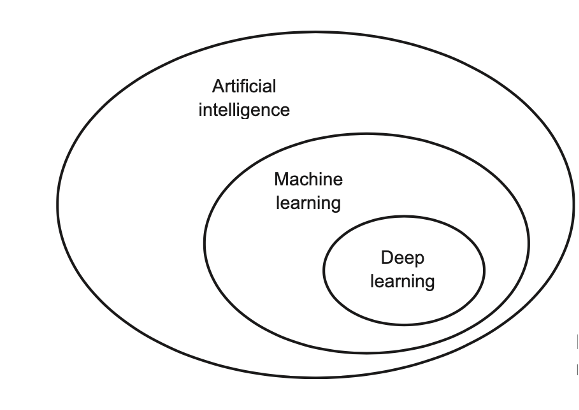
\includegraphics[width=1\textwidth]{1-ia-ml-dl}
    \caption{Intelligence Artificielle, Machin learning et Deep learning.}
    \label{fig:1-ia-ml-dl}
\end{figure}

\subsection{Notion d'apprentissage automatique}
\paragraph{}Dans l'Angleterre victorienne, Lady Ada Lovelace était une amie et collaboratrice de Charles Babbage, l'inventeur de la machine analytique : le premier ordinateur mécanique polyvalent connu. Bien que visionnaire et très en avance sur son temps, l'Analytical Engine n'était pas conçu comme un ordinateur à usage général lorsqu'il a été conçu dans les années 1830 et 1840, car le concept de calcul à usage général n'était pas encore inventé. Il s'agissait simplement d'un moyen d'utiliser des opérations mécaniques pour automatiser certains calculs du domaine de l'analyse mathématique, d'où le nom de moteur analytique. 
\paragraph{}En 1843, Ada Lovelace a fait remarquer à propos de l'invention : « La machine analytique n'a aucune prétention à créer quoi que ce soit. Il peut faire tout ce que nous savons comment lui ordonner de fonctionner... Son rôle est de nous aider à mettre à disposition ce que nous connaissons déjà. Cette remarque a ensuite été citée par le pionnier de l'IA, Alan Turing, comme "l'objection de Lady Lovelace" dans son article historique de 1950 "Computing Machinery and Intelligence",1 qui a présenté le test de Turing ainsi que les concepts clés qui allaient façonner l'IA. Turing citait Ada Lovelace alors qu'il se demandait si les ordinateurs à usage général pouvaient être capables d'apprentissage et d'originalité, et il en est venu à la conclusion qu'ils le pouvaient.
\paragraph{}L'apprentissage automatique découle de cette question : un ordinateur pourrait-il aller au-delà de "ce que nous savons lui ordonner d'exécuter" et apprendre par lui-même comment effectuer une tâche spécifiée ? Un ordinateur pourrait-il nous surprendre ? Plutôt que des programmeurs élaborant des règles de traitement de données à la main, un ordinateur pourrait-il automatiquement apprendre ces règles en examinant les données ?
Cette question ouvre la porte à un nouveau paradigme de programmation. 
\paragraph{}En programmation classique, le paradigme de l'IA symbolique, les humains saisissent des règles (un programme) et des données à traiter selon ces règles, et en sortent des réponses (voir figure 1.2).
\paragraph{}Avec l'apprentissage automatique, les humains saisissent les données ainsi que les réponses attendues des données, et sortent les règles. Ces règles peuvent ensuite être appliquées à de nouvelles données pour produire des réponses originales.

\begin{figure}[h]
    \centering
    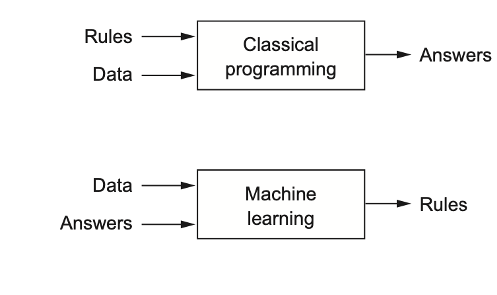
\includegraphics[width=1\textwidth]{1-ml}
    \caption{Machin learning Nouveau paradigme de programmation.}
    \label{fig:1-ml}
\end{figure}

\paragraph{}Un système d'apprentissage automatique est entraîné plutôt qu'explicitement programmé. Il est présenté avec de nombreux exemples pertinents pour une tâche, et il trouve une structure statistique dans ces exemples qui permet finalement au système de proposer des règles pour automatiser la tâche. 
\paragraph{}Par exemple, si vous souhaitez automatiser la tâche d'étiquetage de vos photos de vacances, vous pouvez présenter un système d'apprentissage automatique avec de nombreux exemples d'images déjà étiquetées par des humains, et le système apprendrait des règles statistiques pour associer des images spécifiques à des étiquettes spécifiques.
\paragraph{}Un système d'apprentissage automatique est entraîné plutôt qu'explicitement programmé. Il est présenté avec de nombreux exemples pertinents pour une tâche, et il trouve une structure statistique dans ces exemples qui permet finalement au système de proposer des règles pour automatiser la tâche. Par exemple, si vous souhaitez automatiser la tâche d'étiquetage de vos photos de vacances, vous pouvez présenter un système d'apprentissage automatique avec de nombreux exemples d'images déjà étiquetées par des humains, et le système apprendrait des règles statistiques pour associer des images spécifiques à des étiquettes spécifiques.
\paragraph{}Bien que l'apprentissage automatique n'ait commencé à prospérer que dans les années 1990, il est rapidement devenu le sous-domaine de l'IA le plus populaire et le plus réussi, une tendance stimulée par la disponibilité d'un matériel plus rapide et d'ensembles de données plus volumineux. 
\paragraph{}L'apprentissage automatique est étroitement lié aux statistiques mathématiques, mais il diffère des statistiques de plusieurs manières importantes. Contrairement aux statistiques, l'apprentissage automatique a tendance à traiter de grands ensembles de données complexes (tels qu'un ensemble de données de millions d'images, chacune composée de dizaines de milliers de pixels) pour lesquels une analyse statistique classique telle que l'analyse bayésienne ne serait pas pratique. En conséquence, l'apprentissage automatique, et en particulier l'apprentissage en profondeur, présente relativement peu de théorie mathématique peut-être trop peu - et est orienté vers l'ingénierie. C'est une discipline pratique dans laquelle les idées sont prouvées empiriquement plus souvent que théoriquement.
\paragraph{}Pour resumer, Le machine learning (apprentissage automatique) est une branche de l'intelligence artificielle qui permet à un système informatique d'apprendre à partir de données et d'expériences passées, sans être explicitement programmé. Il s'agit d'une technique d'analyse de données qui utilise des algorithmes pour identifier des modèles et des tendances dans les données, puis les utilise pour faire des prédictions ou des recommandations. Le machine learning est utilisé dans de nombreux domaines, tels que la reconnaissance vocale, la reconnaissance faciale, la détection de fraudes, la recommandation de produits, etc.

\subsection{Notions de Deep learning}
\subsubsection{définition}

\paragraph{}Le deep learning, ou apprentissage profond en français, est une branche de l'intelligence artificielle qui utilise des réseaux de neurones artificiels pour apprendre à partir de données complexes et massives. Il s'agit d'une technique d'apprentissage automatique qui permet aux machines d'apprendre à partir d'un grand nombre de données en les nourrissant à travers des couches de neurones interconnectés \cite{dlp}. 
\paragraph{}Le deep dans  deep learning ne fait référence à aucune sorte de compréhension plus profonde obtenue par l'approche ; il représente plutôt cette idée de couches successives de représentations. Le nombre de couches qui contribuent à un modèle de données est appelé la profondeur du modèle. 
\paragraph{}Dans l'apprentissage profond, ces représentations en couches sont (presque toujours) apprises via des modèles appelés réseaux de neurones, structurés en couches littérales empilées les unes sur les autres. Le terme réseau de neurones fait référence à la neurobiologie, mais bien que certains des concepts centraux de l'apprentissage en profondeur aient été développés en partie en s'inspirant de notre compréhension du cerveau, les modèles d'apprentissage en profondeur ne sont pas des modèles du cerveau. Il n'y a aucune preuve que le cerveau implémente quelque chose comme les mécanismes d'apprentissage utilisés dans les modèles modernes d'apprentissage en profondeur. 
\paragraph{}Le deep learning est utilisé dans de nombreux domaines tels que la reconnaissance d'image, la reconnaissance vocale, la traduction automatique, la prédiction de résultats, etc. Cette technologie est devenue très populaire ces dernières années grâce à ses performances exceptionnelles dans la reconnaissance de formes et dans l'analyse de données complexes.
\paragraph{}Examinons comment un réseau de plusieurs couches de profondeur (voir la figure \ref{fig:1-dl-1} ) transforme l'image d'un chiffre afin de reconnaître de quel chiffre il s'agit.

\begin{figure}[h]
    \centering
    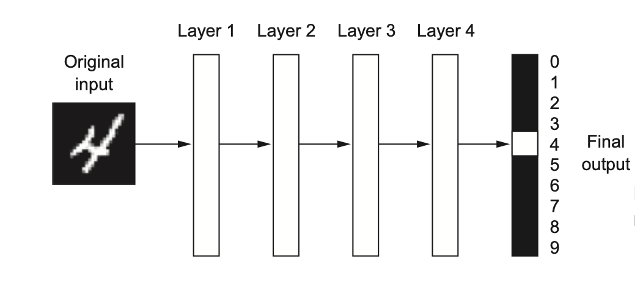
\includegraphics[width=1\textwidth]{1-dl-1}
    \caption{Un Reseau de neurone pour la reconnaissance des caractères.}
    \label{fig:1-dl-1}
\end{figure}

\paragraph{}Comme on peut le voir sur la figure \ref{fig:1-dl-2} , le réseau transforme l'image numérique en représentations de plus en plus différentes de l'image originale et de plus en plus informatives sur le résultat final. On peut  considérer un réseau profond comme une opération de distillation d'informations à plusieurs étapes, où les informations passent par des filtres successifs et sortent de plus en plus purifiées (c'est-à-dire utiles pour certaines tâches).

\begin{figure}[h]
    \centering
    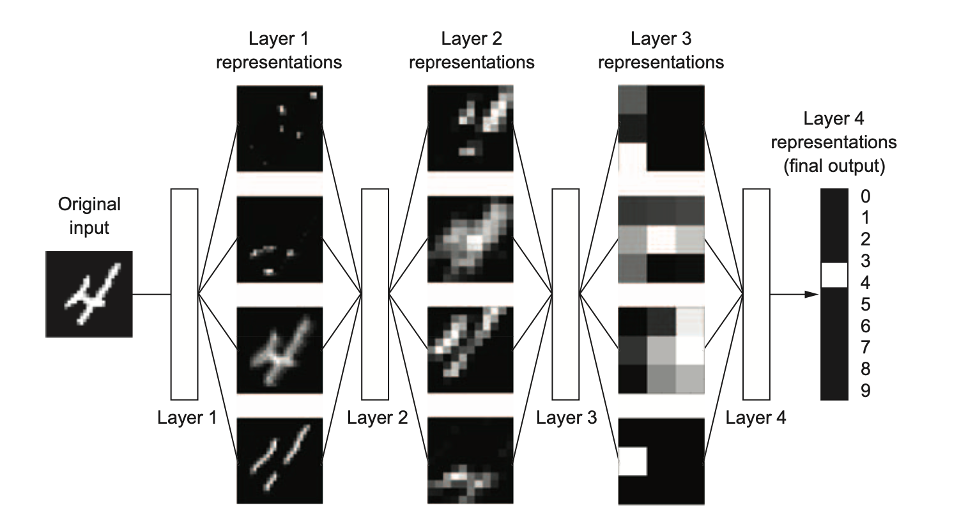
\includegraphics[width=1\textwidth]{1-dl-2}
    \caption{modèle de classification de caractères manuscrits.}
    \label{fig:1-dl-2}
\end{figure}
\paragraph{}

\subsubsection{Fonctionnement}
\paragraph{}La spécification de ce qu'une couche fait à ses données d'entrée est stockée dans les poids de la couche, qui sont essentiellement un ensemble de nombres. En termes techniques, on dirait que la transformation mise en œuvre par une couche est paramétrée par ses poids (voir figure \ref{fig:1-dl-3}). dans  ce contexte, l'apprentissage signifie trouver un ensemble de valeurs pour les pondérations de toutes les couches d'un réseau, de sorte que le réseau mappe correctement les exemples d'entrées sur leurs cibles associées.
Mais voici le problème : un réseau de neurones profonds peut contenir des dizaines de millions de paramètres. Trouver la valeur correcte pour chacun d'eux peut sembler une tâche ardue, d'autant plus que la modification de la valeur d'un paramètre affectera le comportement de tous les autres !
\begin{figure}[h]
    \centering
    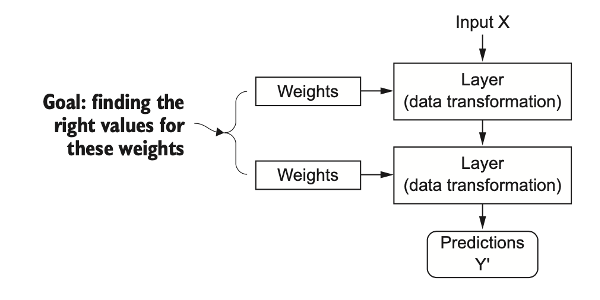
\includegraphics[width=1\textwidth]{1-dl-3}
    \caption{Paramétrisation d’un réseau de neurones}
    \label{fig:1-dl-3}
\end{figure}

\paragraph{}
\paragraph{}

Pour contrôler la sortie d'un réseau de neurones, on doit  être en mesure de mesurer à quelle distance cette sortie (la prédiction, Y’) \cite{dlp}  est de ce que vous attendiez (le résultat attendu, Y). C'est le travail de la fonction de perte du réseau, également appelée fonction objectif. La fonction de perte prend les prédictions du réseau et la véritable cible (ce que vous vouliez que le réseau produise) et calcule un score de distance, capturant la performance du réseau sur cet exemple spécifique (voir figure \ref{fig:1-dl-3}).
\paragraph{}

\begin{figure}[h]
    \centering
    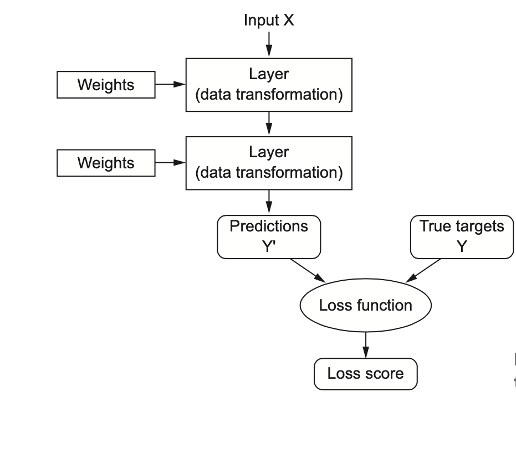
\includegraphics[width=1\textwidth]{1-dl-4}
    \caption{Détermination de la fonction Loss}
    \label{fig:1-dl-4}
\end{figure}

L'astuce fondamentale dans l'apprentissage  profond consiste à utiliser ce score comme un signal de rétroaction pour ajuster un peu la valeur des poids, dans une direction qui abaissera le score de perte pour l'exemple actuel (voir figure \ref{fig:1-dl-5} ). Cet ajustement est le travail de l'optimiseur, qui implémente ce qu'on appelle l'algorithme de rétropropagation : l'algorithme central de l'apprentissage en profondeur. 
\begin{figure}[h]
    \centering
    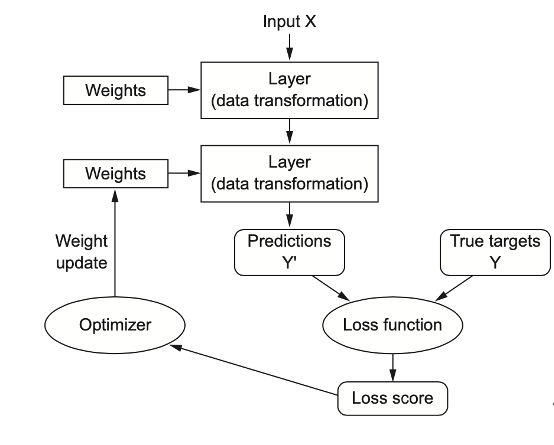
\includegraphics[width=1\textwidth]{1-dl-5}
    \caption{Le Loss Score utilisé pour optimiser le Weigth à  l'entrée}
    \label{fig:1-dl-5}
\end{figure}
\paragraph{}Initialement, les poids du réseau reçoivent des valeurs aléatoires, de sorte que le réseau implémente simplement une série de transformations aléatoires. Naturellement, son rendement est loin de ce qu'il devrait être idéalement, et le score de perte est donc très élevé. Mais avec chaque exemple traité par le réseau, les pondérations sont légèrement ajustées dans la bonne direction et le score de perte diminue. Il s'agit de la boucle d'apprentissage qui, répétée un nombre suffisant de fois (généralement des dizaines d'itérations sur des milliers d'exemples), donne des valeurs de poids qui minimisent la fonction de perte. Un réseau avec une perte minimale est un réseau dont les sorties sont aussi proches que possible des cibles : un réseau entraîné. 
\paragraph{}En résumé, le deep learning implique la collecte et la préparation des données, \cite{dlp}  la construction et l'entraînement du réseau de neurones, l'évaluation du modèle et enfin la prédiction. Le processus de deep learning est souvent itératif, et il peut être nécessaire d'ajuster les paramètres du modèle ou de modifier l'architecture du réseau de neurones pour améliorer les performances du modèle.

\newpage 
\newpage 
\section{deep Learning pour la reconnaissance vocale}

\paragraph{}Dans le domaine de la reconnaissance de locuteur, le Deep Learning est utilisé pour améliorer la précision des systèmes de reconnaissance de la parole en analysant les caractéristiques du signal vocal. Plusieurs méthodes de Deep Learning sont utilisées pour la reconnaissance de locuteur :
\begin{itemize}
    \item \textbf{Réseaux de neurones convolutionnels (CNN)} : Les CNN sont largement utilisés pour l'analyse d'images, mais ils ont également été appliqués à la reconnaissance de locuteur en utilisant des images spectrographiques du signal vocal. Les CNN peuvent extraire des caractéristiques significatives du signal vocal qui peuvent être utilisées pour identifier le locuteur.
    \item \textbf{Réseaux de neurones récurrents (RNN)} : Les RNN sont utilisés pour modéliser des séquences de données, telles que des séquences de phonèmes dans la parole. Les RNN peuvent être utilisés pour identifier le locuteur en analysant les modèles de parole spécifiques à chaque locuteur.
    \item \textbf{Réseaux de neurones profonds (DNN)} : Les DNN sont utilisés pour l'apprentissage en profondeur en utilisant des couches de neurones artificiels. Les DNN ont été utilisés pour la reconnaissance de locuteur en analysant les caractéristiques du signal vocal telles que la fréquence, l'intensité, la durée et les modèles de parole.
    \item \textbf{Réseaux adversaires génératifs (GAN)} : Les GAN sont utilisés pour générer des données synthétiques en imitant les données réelles. Les GAN ont été utilisés pour la reconnaissance de locuteur en générant des images spectrographiques du signal vocal qui peuvent être utilisées pour entraîner des modèles de reconnaissance de locuteur.
\end{itemize}
\paragraph{}Les TDNN (Time-Delay Neural Networks) représentent une architecture de réseaux de neurones artificiels, qui utilisent des couches de neurones à délai temporel pour traiter des données séquentielles ou temporelles. Ces réseaux sont capables de modéliser des dépendances temporelles entre des événements, en prenant en compte l'ordre et le timing des entrées. Les TDNN sont souvent utilisés pour la reconnaissance de la parole, la classification de séries temporelles, la prédiction de séquences, etc.
\paragraph{}En somme, ces techniques et méthodes de Deep Learning permettent d'améliorer la précision de la reconnaissance de locuteur en analysant les caractéristiques du signal vocal de manière plus fine et précise \cite{tdnn}.

\subsection{que représentent les x-vector dans la reconnaissance vocale?}
\paragraph{}Les x-vector sont une représentation numérique de haut niveau d'un segment de signal vocal, qui est utilisée dans la reconnaissance vocale pour l'identification des individus. Les x-vector sont calculés à partir de caractéristiques acoustiques telles que les coefficients cepstraux de fréquence (MFCC) extraits d'un segment de parole \cite{xvectors}.	
\paragraph{}Les x-vector sont généralement extraits en utilisant des réseaux de neurones profonds appelés réseaux de neurones convolutionnels (CNN) et des réseaux de neurones récurrents (RNN), qui sont entraînés à prédire l'identité du locuteur à partir des caractéristiques acoustiques. Le réseau de neurones est ensuite utilisé pour extraire les x-vector à partir de nouvelles données de parole, qui sont ensuite utilisées pour identifier l’individus.
\paragraph{}Les x-vector ont plusieurs avantages par rapport aux méthodes traditionnelles de reconnaissance vocale basées sur les traits acoustiques. Ils peuvent être utilisés pour représenter des segments de parole de longueur variable, sont robustes aux variations de canal et peuvent être utilisés pour l'identification des individus dans des scénarios multi-locuteurs. Les x-vector ont été utilisés avec succès dans de nombreux systèmes de reconnaissance vocale, notamment dans les systèmes de sécurité et de surveillance.

\subsection{que représentent les DNN}

\textbf{Les DNN (Deep Neural Networks)} représentent une classe de modèles de réseaux de neurones artificiels qui sont capables de traiter des données complexes et d'effectuer des tâches de classification, de reconnaissance de motifs, de traitement de langage naturel, etc. Les DNN utilisent plusieurs couches de neurones pour extraire des caractéristiques de plus en plus abstraites à partir des données d'entrée, ce qui leur permet d'apprendre des représentations profondes des données et de réaliser des tâches de manière plus précise et efficace que les modèles de réseaux de neurones plus simples. Les DNN ont trouvé des applications dans de nombreux domaines, notamment la vision par ordinateur, le traitement du langage naturel, la reconnaissance de la parole, la biologie, la médecine, la finance, etc.

\subsection{Les ECAPA-TDNN }
\paragraph{}Les ECAPA-TDNN (Ensemble Classifiers using Adaptive Partitioning Algorithm - Time-Delay Neural Network) sont un type de modèle de classification utilisé en intelligence artificielle et en reconnaissance de formes. Ils combinent les techniques d'ensemble learning (utilisation de multiples classificateurs pour améliorer la précision de la classification) avec les réseaux de neurones à retards temporels (TDNN) pour résoudre des problèmes de classification complexes. Les ECAPA-TDNN sont particulièrement adaptés pour la reconnaissance de formes dans des signaux temporels tels que les signaux audio, les séries chronologiques, les images vidéo, etc. Ils sont largement utilisés dans des domaines tels que la reconnaissance de la parole, la reconnaissance de gestes et la vision par ordinateur \cite{embeddings}.

\subsection{Les ECAPA-TDNN }
\paragraph{}Les PLDA (Probabilistic Linear Discriminant Analysis) sont des modèles d'apprentissage automatique utilisés dans la classification de données. Ils sont principalement utilisés pour l'analyse discriminante linéaire, qui est une méthode statistique qui permet de déterminer la catégorie à laquelle une observation appartient en se basant sur un ensemble de variables prédéfinies. Les PLDA sont souvent utilisés dans le domaine de la reconnaissance vocale pour l'identification des locuteurs, mais peuvent également être appliqués à d'autres types de données. Ils sont considérés comme un outil efficace pour la réduction de dimensionnalité et pour l'analyse des données à grande échelle.

\section{Les bonnes pratiques en matière de reconnaissance vocale}
\paragraph{}Comme pour toute méthode de sécurité, il existe certaines meilleures pratiques de base que les organisations doivent suivre pour s'assurer que les informations de leurs clients ne sont pas en danger \cite{mathworks}.

\begin{itemize}
    \item Établir une méthode d'authentification principale avant toute autre méthode ; cela signifie choisir une forme de validation, qu'il s'agisse d'un code PIN, d'un mot de passe ou d'une biométrie, avant d'accepter d'utiliser plus d'authentifications.
    \item Obtenir le consentement explicite de l'utilisation prévue des utilisateurs pour la mesure de sécurité ; par exemple, accord d'utilisation de la reconnaissance faciale pour permettre les transactions de paiement.
    \item Exiger la méthode d'authentification principale toutes les 72 heures.
    \item Utiliser un pipeline entièrement sécurisé pour toutes les données biométriques et leur manipulation.
    \item Conserver toutes les données biométriques dans un environnement sécurisé et isolé pour empêcher leur acquisition par des fraudeurs.
\end{itemize}
L'utilisation des étapes ci-dessus fournit une excellente base à toute entreprise pour assurer la sécurité des informations de ses clients. Il fournit également une base pour commencer à ajouter plus de niveaux d'authentification afin de créer un système de vérification encore plus puissant.

\section{À quel point la reconnaissance vocale est-elle sécurisée ?}
\paragraph{}La commodité qu'offre la reconnaissance vocale se fait-elle au détriment de la sécurité ? Il y a eu de nombreuses histoires dans les nouvelles sur les pirates capables d'infiltrer les maisons et les entreprises au détriment de leurs propriétaires en utilisant des problèmes de sécurité de reconnaissance vocale. Comme pour toute mesure de sécurité, croire qu'une seule mesure à elle seule est infaillible est imprudent \cite{softjourn}.
\paragraph{}Il reste encore du chemin à parcourir pour parvenir à une identification vocale absolument sécurisée. L'état actuel de la biométrie vocale est vulnérable. Des recherches ont montré que des échantillons de voix provenant de quelque chose comme une vidéo YouTube peuvent être acceptés comme modèles de parole approuvés. Les pirates ont pu enterrer des commandes malveillantes dans du bruit blanc pour contrôler les appareils à commande vocale.
\paragraph{}Selon Lior Atzi, directeur de la gestion des produits chez NICE, deux technologies majeures sont utilisées pour lutter contre la fraude dans l'authentification vocale : la détection de la vivacité et l'authentification continue. 
\paragraph{}La détection de la vivacité, comme son nom l'indique, garantit que l'empreinte digitale ou l'échantillon vocal utilisé est réel. Certaines tentatives pour contrecarrer cette mesure de sécurité sont des voix synthétiques et d'autres implémentations d'intelligence artificielle, mais elles n'ont pas encore suffisamment progressé pour provoquer une menace réelle.
\paragraph{}L'authentification continue vérifie à plusieurs reprises l'identité d'un individu tout au long d'une session, plutôt qu'une seule fois. Cela aide à surmonter les problèmes potentiels tels que les appelants qui changent au milieu d'un appel téléphonique ou d'autres astuces qu'un mauvais acteur pourrait utiliser pour accéder au compte de quelqu'un.


 


\newpage 
\addcontentsline{toc}{section}{Conclusion}
\section*{Conclusion}
\paragraph{}L'authentification vocale rend les connexions aussi simples que parler. Cela peut sembler futuriste, mais c'est la sécurité qui protège les entreprises des violations quotidiennes.
\paragraph{}La reconnaissance vocale est-elle sécurisée ? Oui, la reconnaissance vocale est sécurisée, surtout par rapport aux connexions classiques qui nécessitent un nom d'utilisateur et un mot de passe. Semblable à d'autres biométries, la reconnaissance vocale est plus sécurisée car une personne doit interagir avec un identifiant plutôt que de simplement saisir un code.
\paragraph{}De toute évidence, l'authentification vocale offre de nombreux avantages, tels que des économies de coûts, une sécurité accrue et une expérience client améliorée.
\paragraph{}Cependant, cela vient avec son propre ensemble de défis. Par exemple, parce que la technologie peut être sensible aux bruits et aux signaux parasites.
\paragraph{}Elle reste tout de même un  excellent choix pour accroitre la sécurités des système utilise comme une vérification supplémentaire, car elle ajoute des couches de protection supplémentaires que les codes d'accès manuels pourraient ne pas fournir. L'authentification vocale est bénéfique à la fois pour les clients et pour l'entreprise car elle élimine la frustration associée aux processus de connexion fastidieux.
\paragraph{}La commodité et la sécurité qu'elle offre en font une méthode de vérification dont l'utilisation ne fera qu'augmenter dans tous les secteurs.
\paragraph{}Dans les prochaines décénies, L'authentification par empreinte vocale est susceptible de gagner encore plus en popularité en raison des améliorations de la précision, causées en grande partie par les progrès de l'IA. Cette croissance est également due aux attentes accrues des clients pour un accès rapide et facile à l'information. La biométrie vocale permet un accès rapide, fluide et hautement sécurisé pour une gamme de cas d'utilisation allant des centres d'appels aux applications mobiles et en ligne, en passant par les chatbots, les appareils IoT et l'accès physique.


 
 \chapter{MODELISATION ET LE DEVELOPPEMENT DE NOTRE MODEL D’IA}\label{chap:2}
 \addcontentsline{toc}{section}{Introduction}
\section*{Introduction}
Nous abordons, dans ce chapitre, la présentation de la méthodologie et des choix techniques. Nous voulons mettre en place un modèle de reconnaissance vocal. Ce model sera des réseaux de neurones profonde (DNN). Nous avons vu précédemment qu’il existait plusieurs méthodes de Deep Learning pour la reconnaissance par empreinte vocale. Dans ce chapitre, nous allons effectuer un choix et approfondir la méthode choisie. Nous allons commencer par la méthode de Deep Learning choisie et l’architecture du système que nous voulons mettre en place. Nous aborderons également les matériels ainsi que les technologies utilisées dans la mise en œuvre du modèle. 

\section{Architecture du système}
La finalité de ce travail est de mettre en place un modèle d’IA pour identification et l’authentification par empreinte vocale. L’IA sera ensuite déployée comme un cloud REST API pour permettre à divers client web ou mobile de pouvoir y accéder.  Ainsi l’architecture sera composée de trois parties : 
\begin{enumerate}
    \item le code de paramétrage de l’IA et la gestion du dataset
    \item Le notebook Google Colab pour l’entrainement 
    \item la partie backend pour servir les APIs d’identification et d’authentification. 
\end{enumerate}
Chacune de ces partie joue un rôle spécifique : 
\begin{itemize}
    \item la partie 1 permet de gérer les paramètres d’exécution et gère l’entrainement du model. 
    \item Le notebook va nous permettre de préparer nos données d’entrainer le model, d’effectuer l’inférence et d’exporter le model optimal vers le backend pour servir le cloud API. 
    \item la partie backend va mettre en œuvre un projet Django qui va offrir les différents API d’identification et d’authentification entre autre. 
\end{itemize}

\section{Matériels}
Le code d’entrainement sera exécuté sur Colab qui nous offre une machine linux avec toutes les ressources CPU, GPU nécessaire a une telle opération. 

\begin{figure}[ht]
    \begin{center}
        \centering
        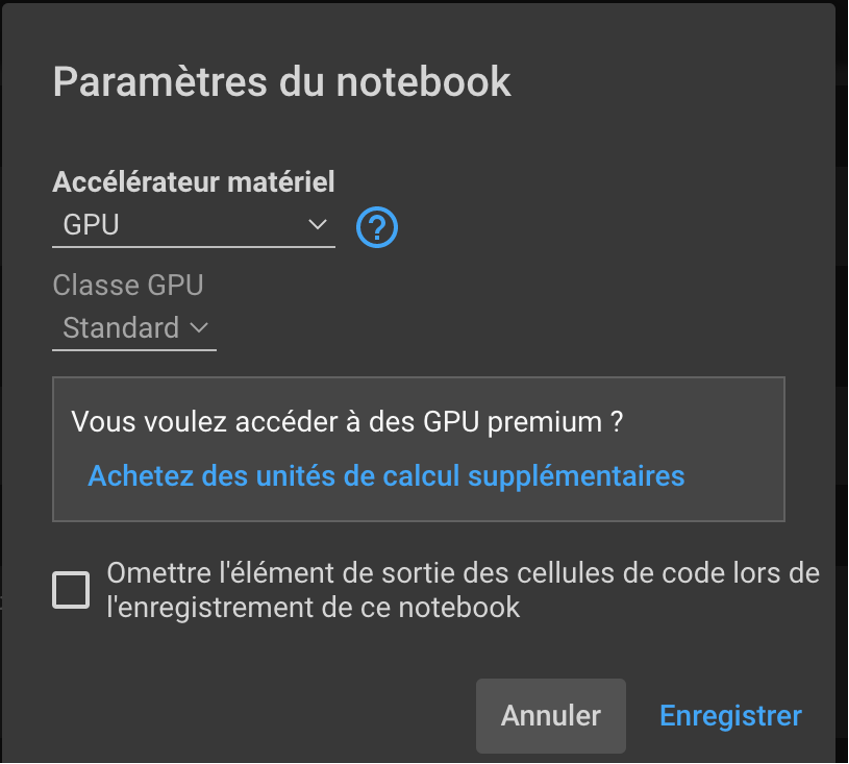
\includegraphics[width=1\textwidth]{2-clab-1}
        \caption{paramètres d'exécution du Colab}
        \label{fig:2-clab-1}
    
    \end{center}
\end{figure}


\begin{figure}
    \begin{center}
        \centering
        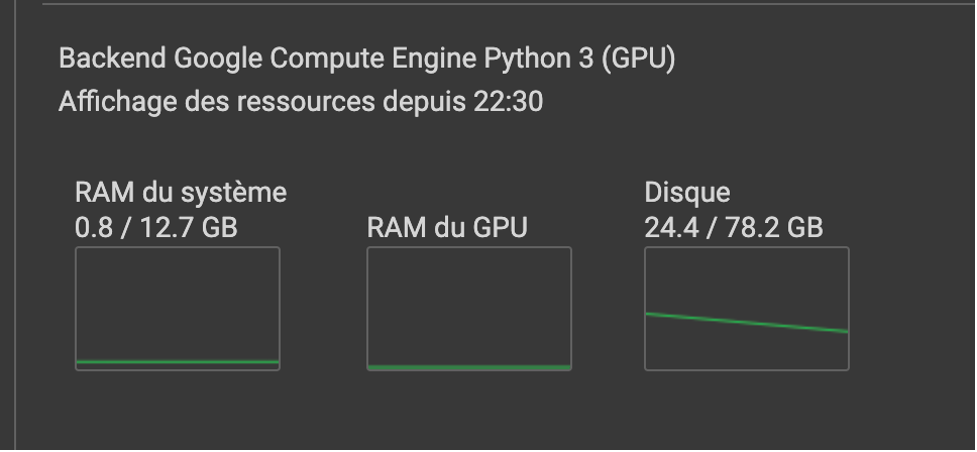
\includegraphics[width=1\textwidth]{2-clab-2}
        \caption{Ressource de l'environnement d'exécution Colab}
        \label{fig:2-clab-2}
        
    \end{center}
\end{figure}




\paragraph{}Le data-set sera sauvegardé sur Google Cloud Storage. En ce qui concerne le backend il sera déployé sur un backend sur le cloud. 

\section{Choix technologique}
\subsection{Définitions }
\paragraph{}\textbf{La reconnaissance de locuteurs}  est utilisée dans de nombreux domaines, tels que la sécurité, la biométrie, la communication et l'analyse de données. Pour réaliser cette reconnaissance, plusieurs méthodes peuvent être utilisées, notamment la reconnaissance automatique de la parole, l'analyse acoustique, la modélisation de la voix et l'apprentissage automatique.
\paragraph{}\textbf{Les x-vectors} sont des vecteurs d'embedding de haut niveau extraits à partir de caractéristiques acoustiques et utilisés pour la reconnaissance automatique de la parole et la vérification du locuteur. Pour extraire les x-vectors, un modèle de réseau de neurones à décalage temporel (TDNN) est souvent utilisé.
Le modèle TDNN pour les x-vectors est entraîné sur de grandes quantités de données de parole pour apprendre à extraire les caractéristiques acoustiques les plus discriminantes pour la reconnaissance du locuteur. Le modèle est ensuite utilisé pour extraire les x-vectors des enregistrements de parole et ces vecteurs sont utilisés pour identifier les locuteurs ou vérifier leur identité.
Nous avons vu dans le chapitre premier que plusieurs méthodes de deep learning pouvaient permettre d’entrainer des modèles de reconnaissance de locuteurs.  Dans le cas de notre étude nous utiliserons les TDNN.
\paragraph{}\textbf{Le TDNN (Time-Delay Neural Networkest)} est une méthode de traitement de la parole qui se concentre sur les caractéristiques temporelles de la parole plutôt que sur les caractéristiques fréquentielles.
Le TDNN utilise une fenêtre temporelle glissante pour extraire des caractéristiques de la parole à partir de segments de durée fixe. Ces caractéristiques sont ensuite traitées par des couches de neurones, chaque couche traitant des caractéristiques de plus en plus abstraites. Le TDNN utilise également des couches de rétropropagation de l'erreur pour ajuster les poids des neurones en fonction de l'erreur de prédiction.
Le TDNN est particulièrement utile pour la reconnaissance de locuteur car il est capable de traiter \textbf{les variations temporelles de la parole, telles que les pauses, les changements de ton et les variations de vitesse. Il peut également être utilisé pour détecter les caractéristiques distinctives de la voix d'un locuteur, telles que la hauteur, la durée et le débit de la parole.}
\paragraph{}\textbf{Le TDNN} est également un type de réseau de neurones convolutif (CNN) qui prend en compte les caractéristiques temporelles dans les données d'entrée. Il utilise des convolutions sur des fenêtres de temps pour extraire des caractéristiques pertinentes de la parole. Le TDNN est ensuite suivi d'une couche d'agrégation globale pour résumer les caractéristiques de la parole dans un vecteur d'embedding de haut niveau (X-Vector).

\paragraph{}En résumé, le TDNN est un outil puissant pour la reconnaissance de locuteur car il peut prendre en compte les informations temporelles de la parole et les variations de la parole dues aux différences de prononciation et de dialecte. Il peut être entraîné à reconnaître les locuteurs à partir d'enregistrements vocaux et peut être utilisé pour prédire le locuteur d'un enregistrement vocal inconnu.

\subsection{Structure }
Les TDNN sont constitués  d'une couche d'entrée, de plusieurs couches cachées et d'une couches de sortie mais ils se différencie de par l'organisation des liaisons inter-couches. Les TDNN introduisent des contraintes qui leurs permettent d'avoir un certain degré d'invariance par décalage temporel et déformation. Celles-ci utilisent trois idées : poids partagés, fenêtre temporelle et délai.
Les poids partagés permettent de réduire le nombre de paramètres du réseau neuronal et induisent ainsi une capacité de généralisation plus importante. Les poids sont partagés suivant la direction temporelle, c'est à dire que pour une caractéristique donnée, la fenêtre associée à celle-ci aura les mêmes poids selon la direction temporelle. De plus cette contrainte entraîne une capacité d'extraire les différences au fur et à mesure du balayage du signal. 
Le concept de fenêtre temporelle implique que chaque neurone de la couche l+1 n'est connecté qu'à un sous ensemble de la couche l (nous n'avons plus une connectivité totale). La taille de cette fenêtre est la même entre deux couches données. Cette fenêtre temporelle permet que chaque neurone n'est qu'une vision locale du signal, il peut être vu comme une unité de détection d'une caractéristique locale du signal.
En plus des deux contraintes précédente nous introduisons des délais entre deux fenêtre successive pour une couche donnée.
De plus chaque couche a deux directions : une direction temporelle et une direction caractéristique \cite{frontiers}.

\begin{figure}[ht]
    \centering
    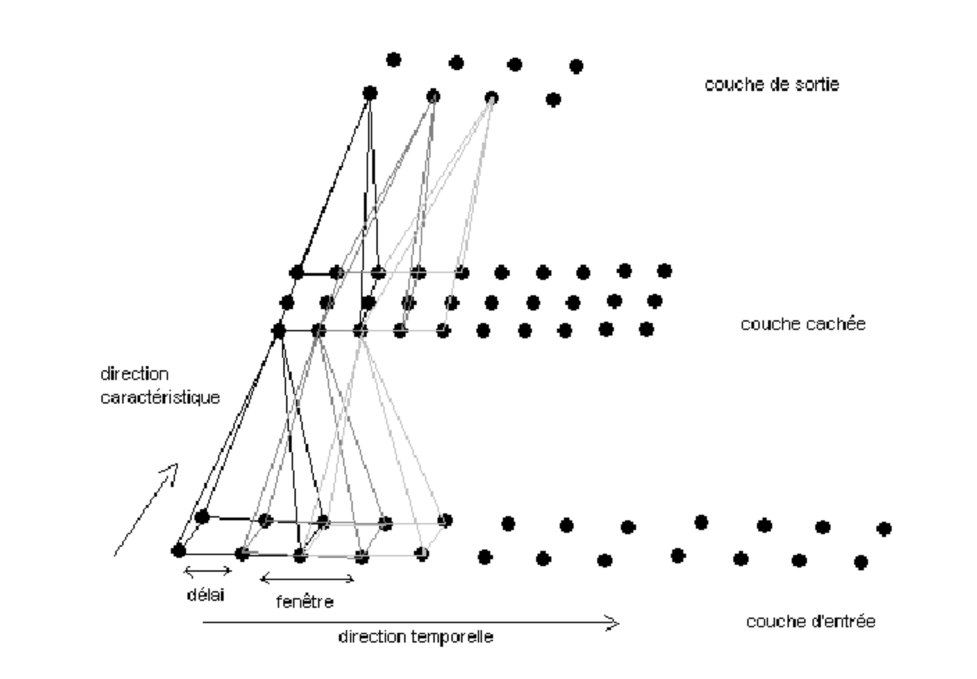
\includegraphics[width=1\textwidth]{2-clab-3}
    \caption{Structure d'un RN de type TDNN}
    % \captionsource{Caption}{ref, cite or free Text}
    \source{The Marvin Project}
    \label{fig:2-clab-3}
\end{figure}

\subsection{Fonctionnement }

\paragraph{}Le but du TDNN est non pas d'apprendre basiquement le signal mais d'extraire les caractéristique de celui-ci. La première couche acquière le signal puis une ou plusieurs couches cachées transforment le signal en des vecteurs de caractéristiques(X-Vectors). Un neurone donné détecte une caractéristique locale de la variation de la courbe. Le champ de vision du neurone est restreint à une fenêtre temporelle limitée. Avec la contrainte des poids partagés, le même neurone est dupliqué dans la direction temps (la même matrice de poids dupliquée) pour détecter la présence ou l'absence de la même caractéristique à différentes places le long du signal. En utilisant plusieurs neurones à chaque position temporelle, le réseau de neurone effectue la détection de caractéristiques différentes : les sorties des différents neurones produisent un nouveau vecteur caractéristique pour la couche supérieure.
\paragraph{}La composante temporelle du signal d'origine est peu à peu éliminée au fur et à mesure de sa transformation en caractéristique par les couches supérieures, pour compenser cette perte d'information on augmente le nombre de neurones dans la direction caractéristique \cite{themarvinproject}.


\addcontentsline{toc}{section}{Conclusion}
\section*{Conclusion}
\paragraph{}Dans ce chapitre, nous avons présenté l’architecture de notre système, les matériels ainsi que les différentes technologies utilisées dans le cadre de notre travail. En ce qui concerne le choix de la méthodologie nous avons opté pour le TDNN. 
\paragraph{}Il faut retenir que le TDNN (Time Delay Neural Network) est une technique d'apprentissage profond qui est largement utilisée pour la reconnaissance de locuteurs. Cette méthode a l'avantage de traiter les signaux acoustiques dans leur temporalité, ce qui permet de prendre en compte les variations temporelles des caractéristiques acoustiques des locuteurs. Le TDNN est également capable de traiter des données de haute dimensionnalité, telles que les signaux audios, en utilisant des réseaux de neurones profonds, ce qui en fait une méthode performante pour la reconnaissance de locuteurs. Dans notre implémentation, il nous permettra d’extraire les x-vectors à partir des caractéristiques acoustiques afin de faire l’identification ou l’authentification du locuteur.

 
\chapter{MATERIELS ET METHODES}\label{chap:3}
 \addcontentsline{toc}{section}{Introduction}
\section*{Introduction}
Ce chapitre est consacré à la modélisation et à l’implémentation de notre model d’IA et du backend Django.  Le model permettre d’offrir deux Rest API (un pour l’authentification et le second pour l’identification). Ainsi n’importe quel client web, mobile ou desktop pourra consommer les Apis.  La modélisation fera l’analyse du contexte qui nous permet de sortir les différentes fonctionnalités que nous allons mettre en exergue à travers un diagramme de cas d’utilisation. Dans l’implémentation, nous abordons les détails relatifs à l’installation des outils de développement et de test, une esquisse du système, Enfin, nous présentons certaines parties du code source.   
%\paragraph{}Ce chapitre est consacré à 
%l  
\section{architecture du système}
\paragraph{}Le TDNN (Time Delay Neural Network) est un type de réseau de neurones récurrent utilisé pour la reconnaissance de la parole et la modélisation de la langue. Il est souvent utilisé dans les systèmes de reconnaissance automatique de la parole, tels que les systèmes de reconnaissance de locuteurs.
\paragraph{}Les x-vectors sont des vecteurs de caractéristiques extraits de l'entrée audio, qui sont utilisés pour la reconnaissance de locuteurs. Les TDNN sont souvent utilisés pour extraire les x-vectors à partir de l'audio.
\paragraph{}L'architecture d'un TDNN utilisé pour extraire les x-vectors est constituée de plusieurs couches de neurones, chacune avec une taille de fenêtre différente. Chaque couche est composée de plusieurs neurones qui sont connectés à des entrées audio avec un retard temporel.
\paragraph{}Le retard temporel est utilisé pour permettre au réseau de traiter des informations audio qui se produisent à différents moments dans le temps. Par exemple, une couche peut être configurée pour traiter des informations audio qui ont été enregistrées 100 millisecondes avant l'instant actuel, tandis qu'une autre couche peut traiter des informations audio enregistrées 200 millisecondes avant l'instant actuel voir figure \ref{fig:2-clab-3}.
\paragraph{}Les sorties de chaque couche sont ensuite combinées pour produire un vecteur de caractéristiques global, qui est utilisé comme x-vector pour la reconnaissance de locuteurs.
\paragraph{}En résumé, l'architecture d'un TDNN utilisé pour extraire les x-vectors est généralement constituée de plusieurs couches de neurones, chacune avec une taille de fenêtre différente et connectée à des entrées audio avec un retard temporel. Les sorties de chaque couche sont combinées pour produire un vecteur de caractéristiques global, qui est utilisé comme x-vector pour la reconnaissance de locuteurs.

\section{Le model}
\paragraph{}Tel que nous l’avons énoncé dans les parties précédentes, De nombreux modèles neuronaux peuvent être utilisés pour aborder ce type de tâche. Dans cette étude, nous nous concentrerons sur un classificateur TDNN (xvector).
\paragraph{}Comme le montre la figure ci-dessous, l’architecture TDNN est basée sur la topologie à vecteur x (xvector), et introduit plusieurs améliorations pour les IA dans le domaine du traitement des signaux vocaux.
\paragraph{}La couche de pooling utilise un mécanisme d'attention dépendant du canal et du contexte, ce qui permet au réseau d'attirer l'attention sur différents frames par canal. Des blocs SqueezeExcitation unidimensionnels (SE) redimensionnent les canaux des cartes de caractéristiques de niveau de frame intermédiaires pour insérer des informations de contexte global dans les blocs de convolution qui fonctionnent localement. Ensuite, l'intégration de blocs Res2 unidimensionnels améliore les performances tout en réduisant simultanément le nombre total de paramètres en utilisant des convolutions groupées de manière hiérarchique.
\paragraph{}Enfin, l'agrégation de fonctionnalités multi-couches (MFA) fusionne des informations complémentaires avant le pooling de statistiques en concaténant la carte de caractéristiques de niveau de frame finale avec des cartes de caractéristiques intermédiaires de couches précédentes.
\paragraph{}Le réseau est entraîné en optimisant la perte AAMsoftmax sur les identités de locuteurs dans le corpus d'entraînement. L'AAM-softmax est une amélioration puissante par rapport à la perte softmax régulière dans le contexte des problèmes de classification et de vérification fine. Il optimise directement la distance cosinus entre les embeddings de locuteur.


\begin{figure}[h]
    \centering
    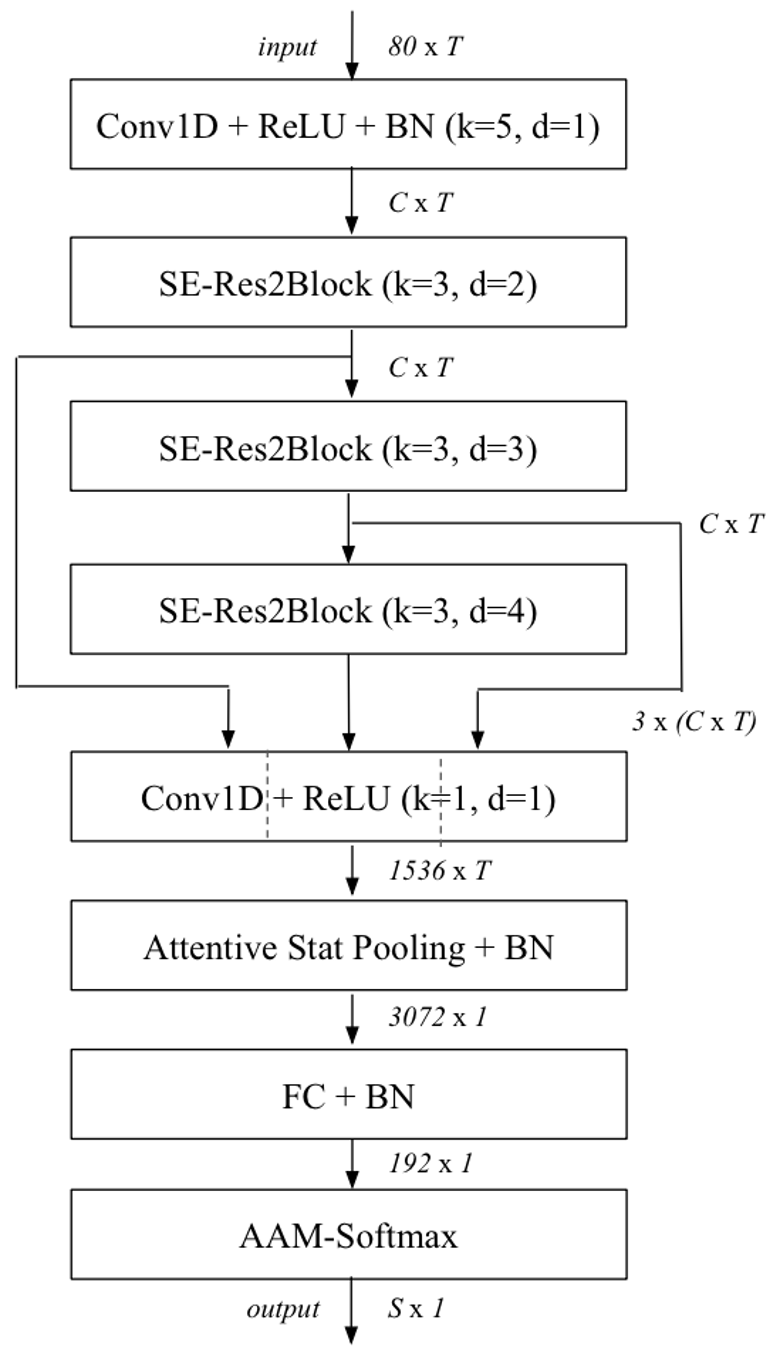
\includegraphics[width=0.5\textwidth]{3chap1}
    \caption{Structure d'un RN de type TDNN}
    \label{fig:3chap1}
\end{figure}
\paragraph{}


\section{Les données d'entrainement}
L’entrainement se fera avec un petit ensemble de données open source appelé minilibrispeech à laquelle nous avons ajouté des données vocales d’un certain nombre de personnalités politiques et médias. Tous les fichiers vocaux sonnt au format .flac, channel Mono et de frequence 16 KHz.

\begin{figure}[h]
    \centering
    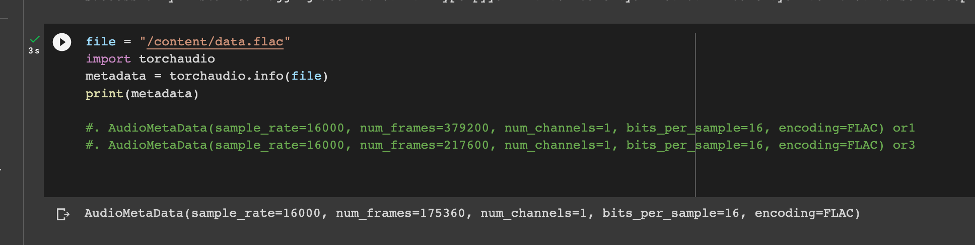
\includegraphics[width=1\textwidth]{3chap2}
    \caption{caractéristiques des enregistrements vocaux}
    \label{fig:3chap2}
\end{figure}
\paragraph{}Nous avons ainsi, un dataset d’une trentaine d’empreinte vocale, qui ne contient que quelques heures de données de formation. Nous avons aussi mis en place un data pipeline qui à partir d’un API Rest peux servir à étendre le dataset. 


\begin{figure}[h]
    \centering
    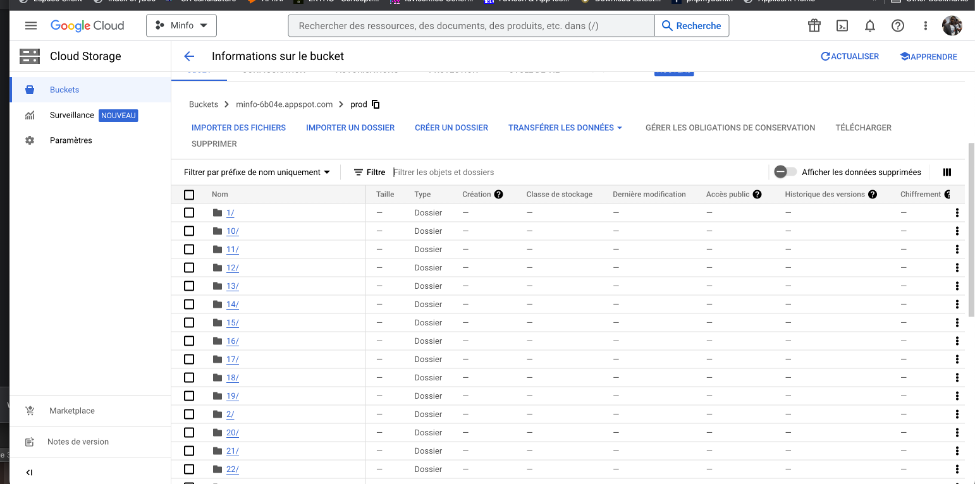
\includegraphics[width=1\textwidth]{3chap3}
    \caption{Le dataset dansle bucket Cloud Storage}
    \label{fig:3chap3}
\end{figure}


\begin{figure}[h]
    \centering
    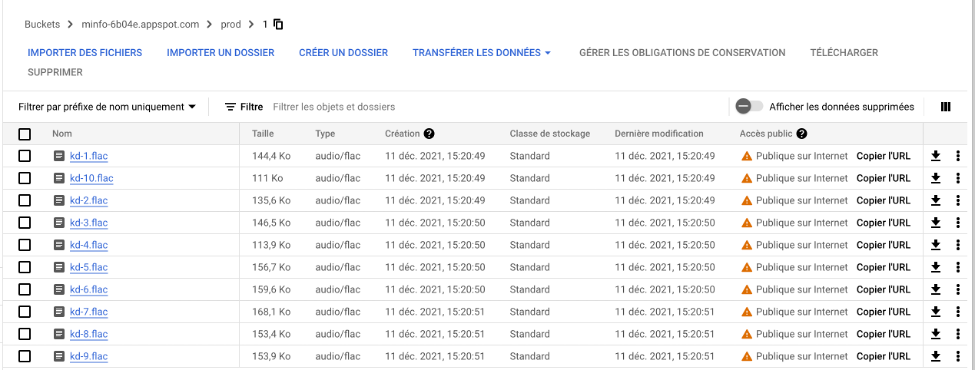
\includegraphics[width=1\textwidth]{3chap4}
    \caption{enregistrementsvocaux d'un seul utilisateur}
    \label{fig:3chap4}
\end{figure}

\section{Le code}
Pour l’entrainement, on va cloner le répertoire  \href{ https://github.com/kadersaka/minfo_speaker_identification}{github.com/kadersaka/minfo-speaker-identification}. On y trouve un ensemble de fichiers et de dossiers, dont :

\begin{itemize}
    \item \textbf{train.py }: le fichier de code principal, décrit l'ensemble du processus d’entrainement.
    \item \textbf{train.yaml }: le fichier d'hyperparamètres, définit tous les paramètres d'exécution.
	\item \textbf{custom-model.py } : un fichier contenant la définition d'un module PyTorch dont on aura besoin pour l’inférence.
	\item \textbf{mini-librispeech-prepare.py} : si nécessaire, télécharge et prépare les manifestes de données si elles ne sont pas encore dans l’environnement d’entrainement.
\end{itemize}
Pour entrainer le modèle speaker-id, on va exécuter la commande :

\section{Installations}
La première chose à faire est de créer un notebook Colab.  Ensuite, nous allons activer l’exécution en mode GPU car nous en auront besoin pour l’entrainement. Puis il faudra cloner le code du répertoire GitHub ci-dessus; (voir figure \ref{fig:3chap5}).
\begin{figure}[h]
    \centering
    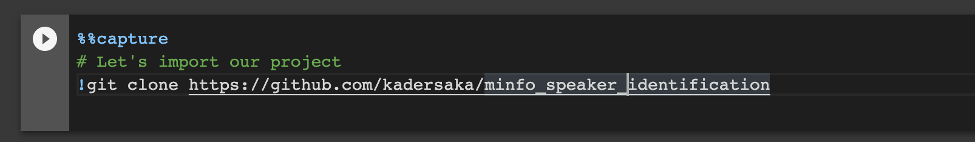
\includegraphics[width=1\textwidth]{3chap5}
    \caption{enregistrementsvocaux d'un seul utilisateur}
    \label{fig:3chap5}
\end{figure}
Ensuite il faudra installer la librairie SpeechBrain (voir figure \ref{fig:3chap6}).
\begin{figure}[h]
    \centering
    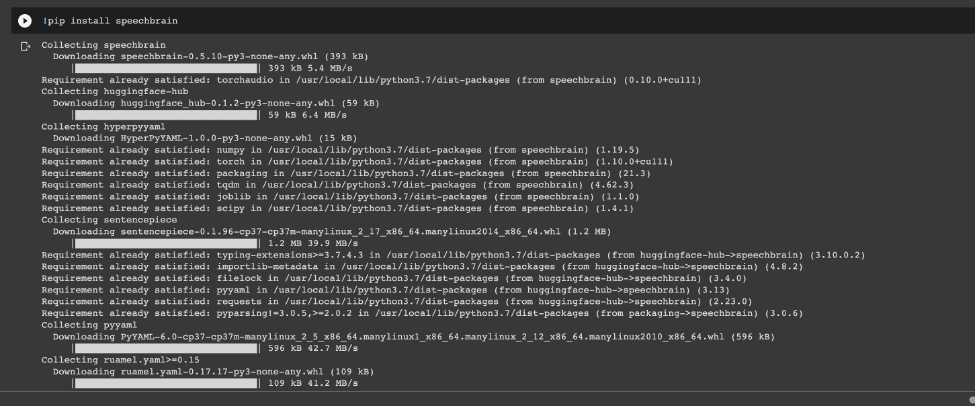
\includegraphics[width=1\textwidth]{3chap6}
    \caption{enregistrementsvocaux d'un seul utilisateur}
    \label{fig:3chap6}
\end{figure}

\section{Preparation des données}
A cette étape la première chose à faire est de donner les autorisations au fichier Colab de pouvoir accéder au Bucket du Cloud Storage pour récupérer le dataset. Ensuite, nous utilisons GsUtils pour la gestion des données du Bucket, notamment leur copie de cloud Storage vers l’environnement local du Colab (voir figure \ref{fig:3chap7}).

\begin{figure}[h]
    \centering
    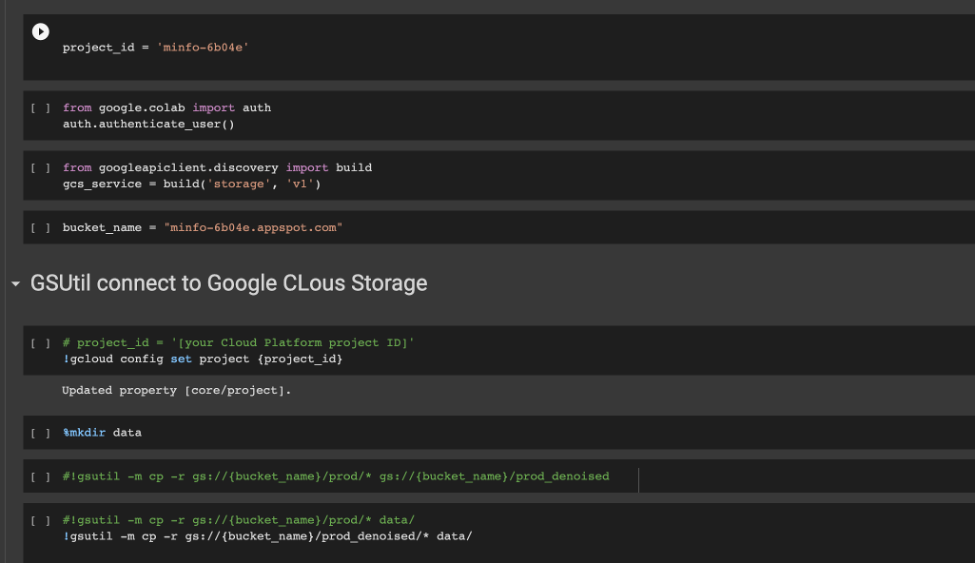
\includegraphics[width=1\textwidth]{3chap7}
    \caption{récupération des données}
    \label{fig:3chap7}
\end{figure}
Après avoir récupéré le dataset, nous pouvons maintenant préparer les données.  L'objectif de la préparation des données est de créer les fichiers manifestes de données. Ces fichiers indiquent à SpeechBrain où trouver les données audio et leur classification au niveau de l'énoncé correspondante. Ce sont des fichiers texte écrits dans les formats populaires CSV et JSON  (voir figure \ref{fig:3chap8}).
\begin{figure}[h]
    \centering
    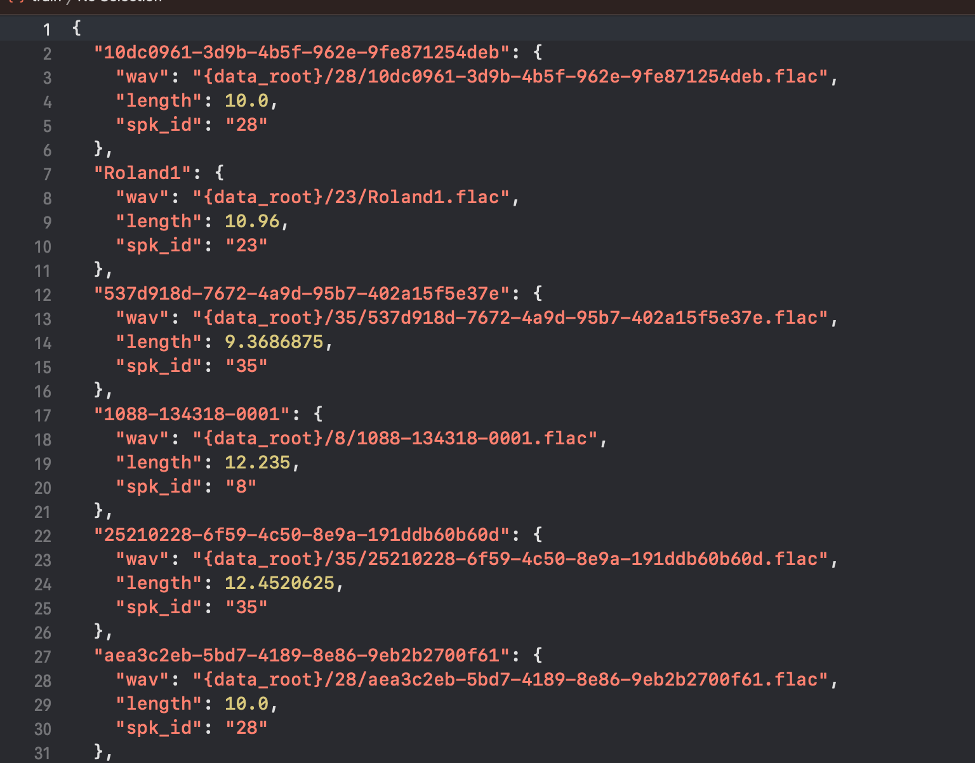
\includegraphics[width=1\textwidth]{3chap8}
    \caption{Fichier manifestes d'entrainement}
    \label{fig:3chap8}
\end{figure}

Comme vous pouvez le voir, nous avons une structure hiérarchique spécifiant tous les champs nécessaires à la tâche adressée. Par exemple, nous rapportons le chemin de l'enregistrement vocal, sa durée en secondes (nécessaire si nous voulons trier les phrases avant de créer les mini-lots) et l'identité (ID) du locuteur dans l'enregistrement donné.
Il faut préciser qu’a cette étape le dataset est divise en trois partitions, chacun avec son fichier manifest :
\begin{itemize}
    \item le premier pour les l’entrainement
    \item le second pour les test
    \item et le troisième pour la validation du model
\end{itemize}

\section{Entrainement du modèle TDNN}

Nous allons former le modèle basé sur TDNN utilisé pour les X-Vector. La mise en commun statistique est utilisée au-dessus des couches convolutives (CNN) pour convertir un vocal de longueur variable en incorporations de longueur fixe. Les parametres sont sur le fichier train.yaml

\begin{figure}[h]
    \centering
    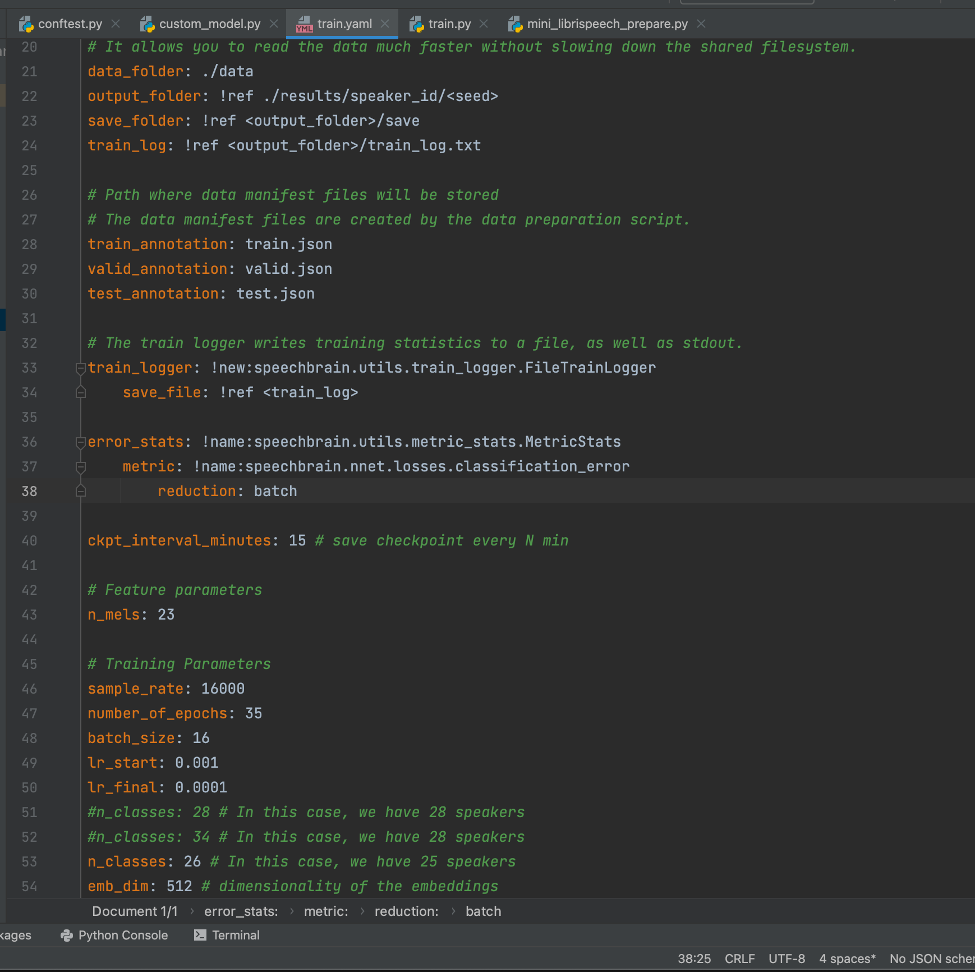
\includegraphics[width=1\textwidth]{3chap9}
    \caption{Fichier des paramètres d'entrainement}
    \label{fig:3chap9}
\end{figure}
Dans ce fichier  (voir figure \ref{fig:3chap9}):
\begin{itemize}
    \item Dans la première partie, nous spécifions quelques paramètres de base, tels que le seed, le chemin du dossier qui contiendra nos fichiers vocaux et le chemin du dossier de sortie (voir figure \ref{fig:3chap10}):
    \begin{figure}[h]
		\centering
		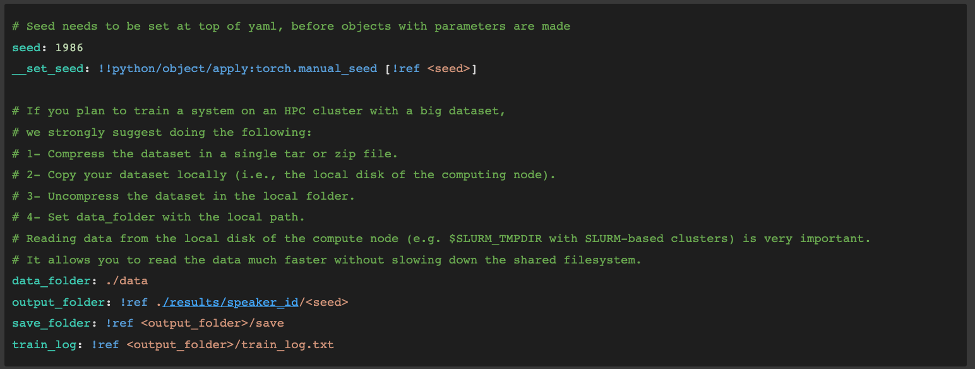
\includegraphics[width=1\textwidth]{3chap10}
		\caption{paramètres de base d'entrainement}
		\label{fig:3chap10}
	\end{figure}
    \item Nous spécifions ensuite le chemin des fichiers manifestes de données pour l’entrainement, la validation et le test voir figure \ref{fig:3chap11}):
	\begin{figure}[h]
		\centering
		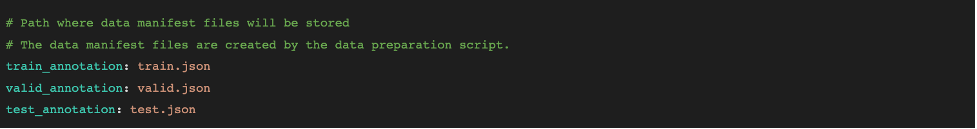
\includegraphics[width=1\textwidth]{3chap11}
		\caption{paramètres des chemins des fichiers manifestes}
		\label{fig:3chap11}
	\end{figure}
	\\Ces fichiers seront créés automatiquement lors de l'appel du script de préparation des données (mini\_librispeech\_prepare.py) à partir du fichier d’entrainement (train.py).
	\item Ensuite, nous configurons le train\_logger et déclarons les objets error\textunderscore stats qui recueilleront des statistiques sur le taux d'erreur de classification (voir figure \ref{fig:3chap12}):
	\begin{figure}[h]
		\centering
		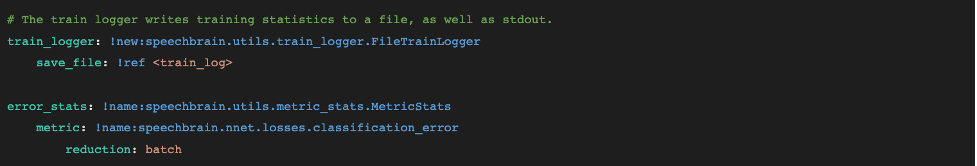
\includegraphics[width=1\textwidth]{3chap12}
		\caption{paramètres des chemins des fichiers manifestes}
		\label{fig:3chap12}
	\end{figure}
	
	\item Nous pouvons maintenant spécifier certains hyperparamètres d'entraînement tels que le nombre d'époques, la taille du lot, le taux d'apprentissage, le nombre d'époques et la dimensionnalité d'intégration (voir figure \ref{fig:3chap13}).
	\begin{figure}[h]
		\centering
		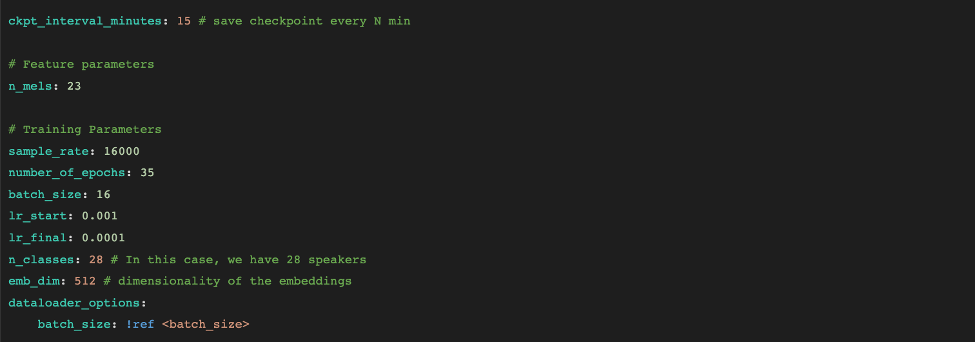
\includegraphics[width=1\textwidth]{3chap13}
		\caption{Autres paramètres}
		\label{fig:3chap13}
	\end{figure}

\end{itemize}

La variable ckpt\_interval\_minutes peut être utilisée pour enregistrer des points de contrôle toutes les N minutes au cours d'une période d'entraînement. Dans certains cas, une époque peut prendre plusieurs heures, et enregistrer périodiquement le point de contrôle est une bonne pratique sûre.  
Nous pouvons maintenant définir les modules les plus importants qui sont nécessaires pour former notre modèle (voir figure \ref{fig:3chap14})

\begin{figure}[h]
	\centering
	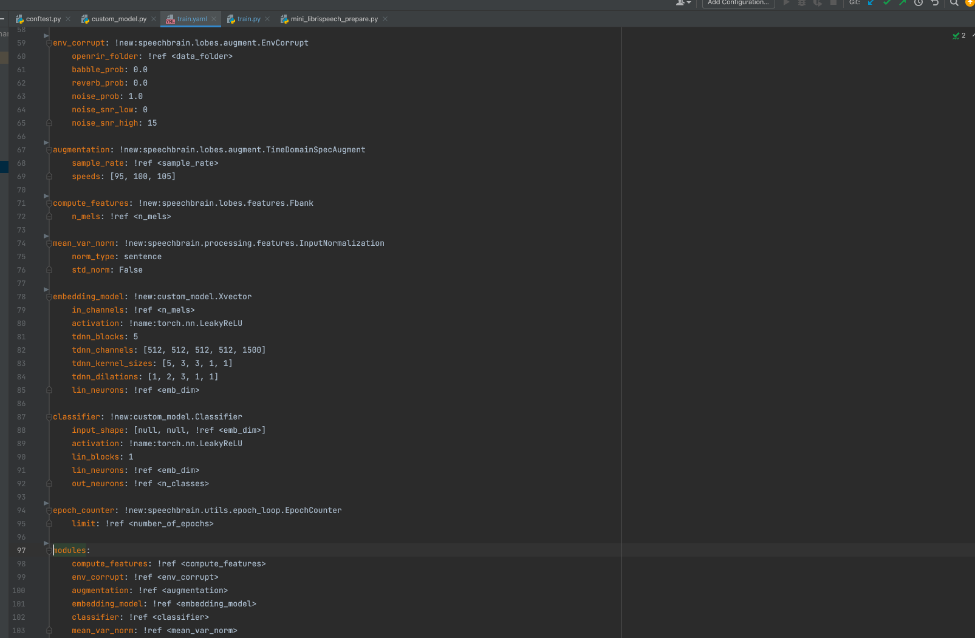
\includegraphics[width=1\textwidth]{3chap14}
	\caption{Paramètres d'augmentation des données avec les bruits}
	\label{fig:3chap14}
\end{figure}

La partie d'augmentation est basée à la fois sur env\_corrupt (qui ajoute du bruit et de la réverbération) et augmentation (qui ajoute des pertes de temps/fréquence et un changement de vitesse). 
Nous terminons la spécification des hyperparamètres avec la déclaration de l'optimiseur, de l'ordonnanceur du taux d'apprentissage et du pointeur de contrôle :
\begin{figure}[h]
	\centering
	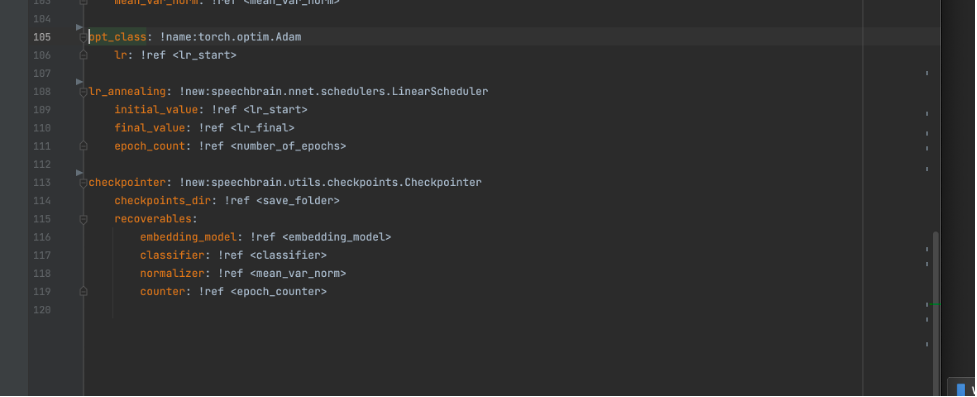
\includegraphics[width=1\textwidth]{3chap15}
	\caption{Paramètres d'augmentation des données avec les bruits}
	\label{fig:3chap15}
\end{figure}

Dans notre  cas, nous utilisons Adam comme optimiseur et une décroissance linéaire du taux d'apprentissage sur les 15 époques.
Adam (Adaptive Moment Estimation) est un optimiseur très populaire pour l'apprentissage profond, car il combine les avantages de deux autres optimiseurs, à savoir la descente de gradient stochastique (SGD) avec moment et la méthode d'estimation adaptative de la moyenne du carré des gradients (RMSProp). L'optimiseur Adam est très efficace pour résoudre des problèmes de gradient évanescents ou explosifs, car il utilise des moments d'ordre supérieur pour adapter le taux d'apprentissage pour chaque paramètre.
En pratique, l'utilisation de la décroissance linéaire du taux d'apprentissage avec l'optimiseur Adam peut améliorer la stabilité et la convergence du modèle, en particulier pour les problèmes de grande envergure avec des données complexes. Cependant, il est important de noter que le taux d'apprentissage doit être choisi avec soin, car une décroissance trop rapide peut conduire à une convergence lente ou à des minima locaux, tandis qu'une décroissance trop lente peut entraîner une instabilité ou une divergence.
Voici donc comment les objets, les fonctions et les hyperparamètres déclarés dans le fichier yaml sont utilisés dans train.py pour implémenter le classifieur.
Parcourrons maintenant le fichier principal train.py (voir figure \ref{fig:3chap16}):

\begin{figure}[h]
	\centering
	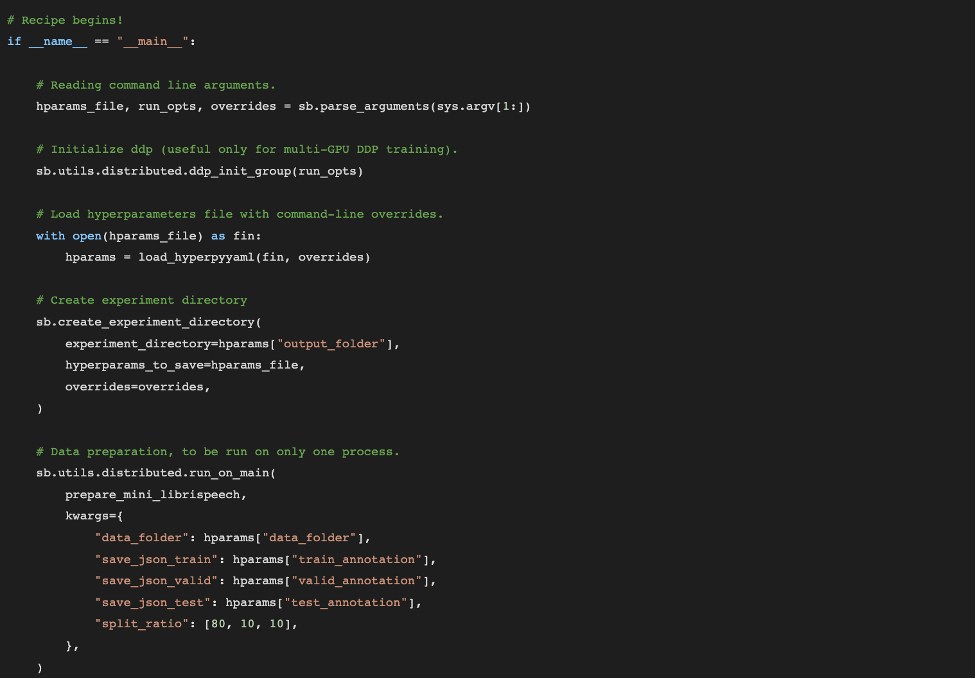
\includegraphics[width=1\textwidth]{3chap16}
	\caption{Code d'entrainement}
	\label{fig:3chap16}
\end{figure}


Nous effectuons ici quelques opérations préliminaires telles que l'analyse de la ligne de commande, l'initialisation des données distribuées en parallèle (nécessaire si plusieurs GPU sont utilisés), la création du dossier de sortie et la lecture du fichier yaml afin de récupérer les paramètres par défaut.
Après lecture du fichier yaml avec load\_hyperpyyaml, tous les objets déclarés dans les fichiers d'hyperparamètres sont initialisés et disponibles sous forme de dictionnaire (ainsi que les autres fonctions et paramètres rapportés dans le fichier yaml). Par exemple, nous aurons hparams['embedding\_model'], hparams['classifier'], hparams['batch\_size'], etc.
Nous exécutons également le script de préparation des données prepare\_mini\_librispeech qui crée les fichiers manifestes de données(distribuées à 80\% pour l'entrainement, 10\% pour la validation, et 10\% pour les tests). Il est encapsulé avec sb.utils.distributed.run\_on\_main car cette opération écrit les fichiers manifestes sur le disque.
\\Nous appelons ensuite la fonction qui crée les objets de l'ensemble de données pour la formation, la validation et le test.

\begin{figure}[h]
	\centering
	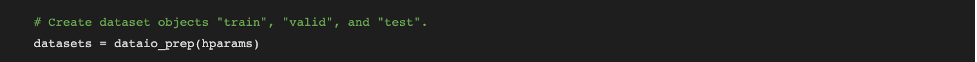
\includegraphics[width=1\textwidth]{3chap17}
	\caption{commande de separation des données}
	\label{fig:3chap17}
\end{figure}

\begin{figure}[h]
	\centering
	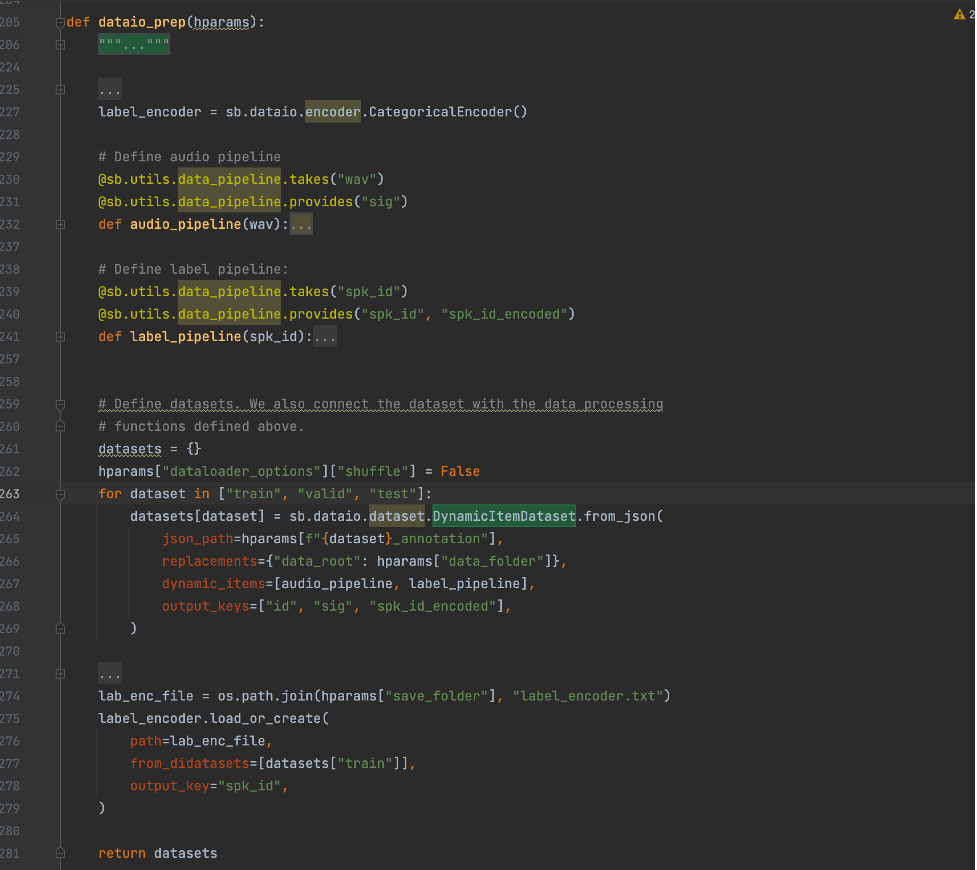
\includegraphics[width=1\textwidth]{3chap18}
	\caption{Code de separation des données}
	\label{fig:3chap18}
\end{figure}

La première partie est juste une déclaration de CategoricalEncoder qui sera utilisée pour convertir les étiquettes catégorielles en leurs index correspondants.
Nous exposons ensuite  les fonctions de traitement audio et label.
La fonction  audio\_pipeline prend le chemin d’un signal audio (wav) et le lit. Il renvoie un objet tensor contenant la phrase vocale lue. L'entrée en paramètre de cette fonction (c'est-à-dire le fichier wav) doit avoir le même nom que la clé correspondante dans le fichier manifeste de données généré:
Ex : 
\begin{figure}[h]
	\centering
	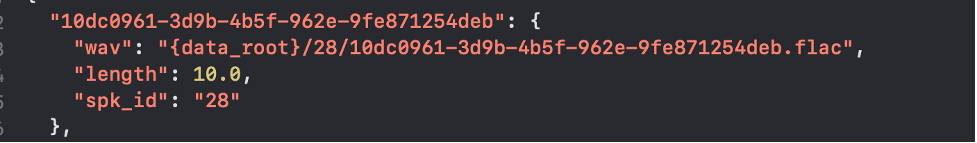
\includegraphics[width=1\textwidth]{3chap19}
	\caption{ligne du fichier manifeste}
	\label{fig:3chap19}
\end{figure}

De même, nous définissons une autre fonction appelée label\_pipeline pour traiter les étiquettes au niveau de l'énoncé et les mettre dans un format utilisable par le modèle défini. La fonction lit la chaîne spk\_id définie dans le fichier JSON et l'encode avec l'encodeur catégoriel.
Nous créons ensuite un objet de type DynamicItemDataset et le connectons aux fonctions de traitement définies ci-dessus. Nous définissons les clés de sortie souhaitées à exposer. Ces clés seront disponibles dans la classe brain dans la variable batch comme :
\begin{itemize}
    \item batch.id
    \item lot.sig
    \item lot.spk\_id\_encoded
\end{itemize}

La dernière partie de la fonction est dédiée à l'initialisation de l'encodeur d'étiquettes. L'encodeur d'étiquettes prend en entrée le jeu de données d'apprentissage et attribue un index différent à toutes les entrées spk\_id trouvées. Ces index correspondront aux index de sortie du classifieur.
Après la définition des jeux de données, la fonction main peut procéder à l'initialisation et à l'utilisation de la classe brain :

\begin{figure}[h]
	\centering
	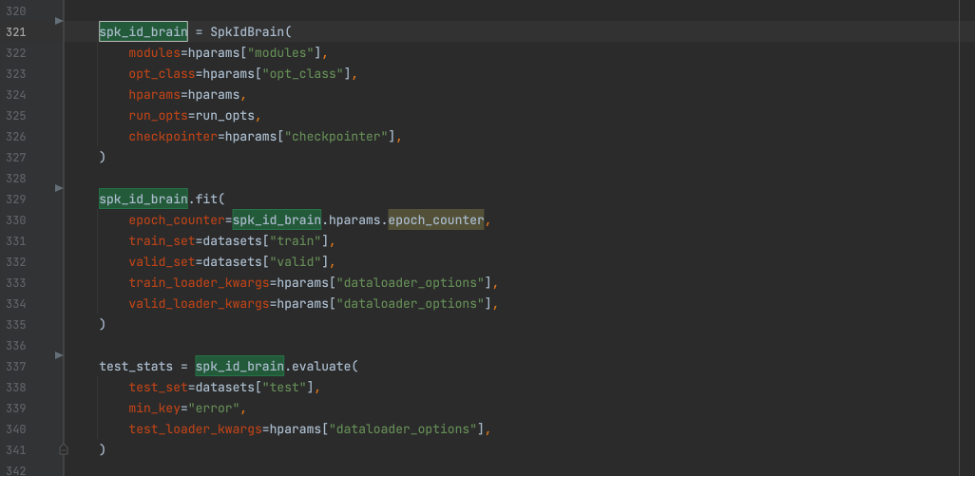
\includegraphics[width=1\textwidth]{3chap20}
	\caption{Classe Brain}
	\label{fig:3chap20}
\end{figure}

La méthode d'ajustement effectue l’entrainement, tandis que le test est effectué avec celui d'évaluation. Les chargeurs de données d'entraînement et de validation sont fournis en entrée de la méthode d'ajustement, tandis que l'ensemble de données de test est introduit dans la méthode d'évaluation.
Examinons maintenant les méthodes les plus importantes définies dans la classe brain:

\subsection*{Les Calculateurs}
Commençons par la fonction forward, qui définit tous les calculs nécessaires pour transformer l'audio d'entrée en prédictions de sortie.

\begin{figure}[h]
	\centering
	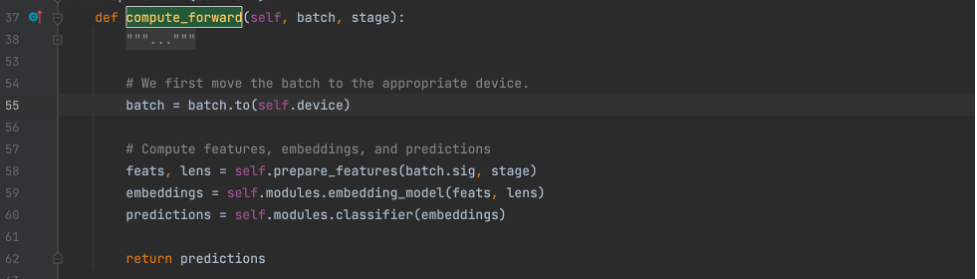
\includegraphics[width=1\textwidth]{3chap21}
	\caption{compute forward}
	\label{fig:3chap21}
\end{figure}

Dans ce cas, la chaîne de calcul est très simple. Nous plaçons simplement le lot sur le bon appareil et calculons les caractéristiques acoustiques. Nous traitons ensuite les caractéristiques avec l'encodeur TDNN qui produit un objet tensor de taille fixe (notre. X-Vector). Ce dernier alimente un classifieur qui sort les probabilités a posteriori sur les N classes (ici les 31 locuteurs). L'augmentation des données est ajoutée dans la méthode prepare\_features :

\begin{figure}[h]
	\centering
	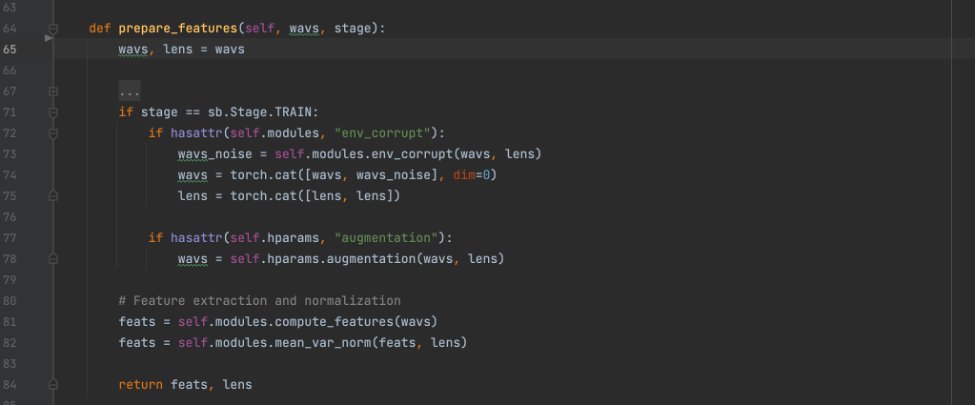
\includegraphics[width=1\textwidth]{3chap22}
	\caption{augmentation des données }
	\label{fig:3chap22}
\end{figure}

En particulier, lorsque la corruption (Fichiers parasites sonores) de l'environnement est déclarée dans le fichier yaml, nous concaténons dans le même lot la version propre et la version augmentée des signaux parasites.
Cette approche double la taille du lot, mais elle implémente un régularisateur très puissant. Le fait d'avoir à la fois la version propre et la version bruyante du signal dans le même lot force le gradient à pointer dans une direction de l'espace des paramètres qui est robuste contre les distorsions du signal.

\subsection*{Objectifs de calcul}
Intéressons-nous maintenant à la méthode compute\_objectives qui prend en entrée les cibles, les prédictions, et estime une fonction de perte :

\begin{figure}[h]
	\centering
	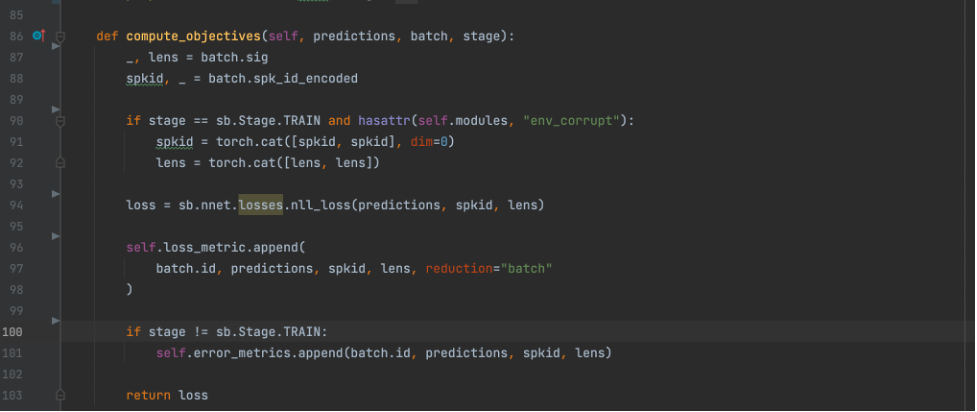
\includegraphics[width=1\textwidth]{3chap23}
	\caption{definition de la fonction de perte}
	\label{fig:3chap23}
\end{figure}
Les prédictions en entrée sont celles calculées dans la méthode directe. La fonction de coût est évaluée en comparant ces prédictions avec les étiquettes cibles. 

\subsection*{Les autres méthodes}
Au-delà de ces deux fonctions importantes, nous avons d'autres méthodes qui sont utilisées par l’IA. Le on\_state\_starts est appelé au début de chaque époque et il est utilisé pour configurer les trackers de statistiques. Le on\_stage\_end est appelé à la fin de chaque étape (par exemple, à la fin de chaque période d'entraînement) et s'occupe principalement de la gestion des statistiques, du recuit du taux d'apprentissage et des points de contrôle. 
\\Pour démarrer l’entraînement nous allons exécuter le code suivant :  
\textbf{python train.py train.yaml --number\_of\_epochs=15}

nous pouvons y passer des paramètres qui vont overrider les paramètres par défaut énoncés sur le fichier train.yaml
On observe sur la console que les pertes de validation et d’entrainement (loss function) diminuent très rapidement dans les premières époques. Ensuite, nous voyons essentiellement quelques améliorations mineures et des oscillations de performances.
\begin{figure}[h]
	\centering
	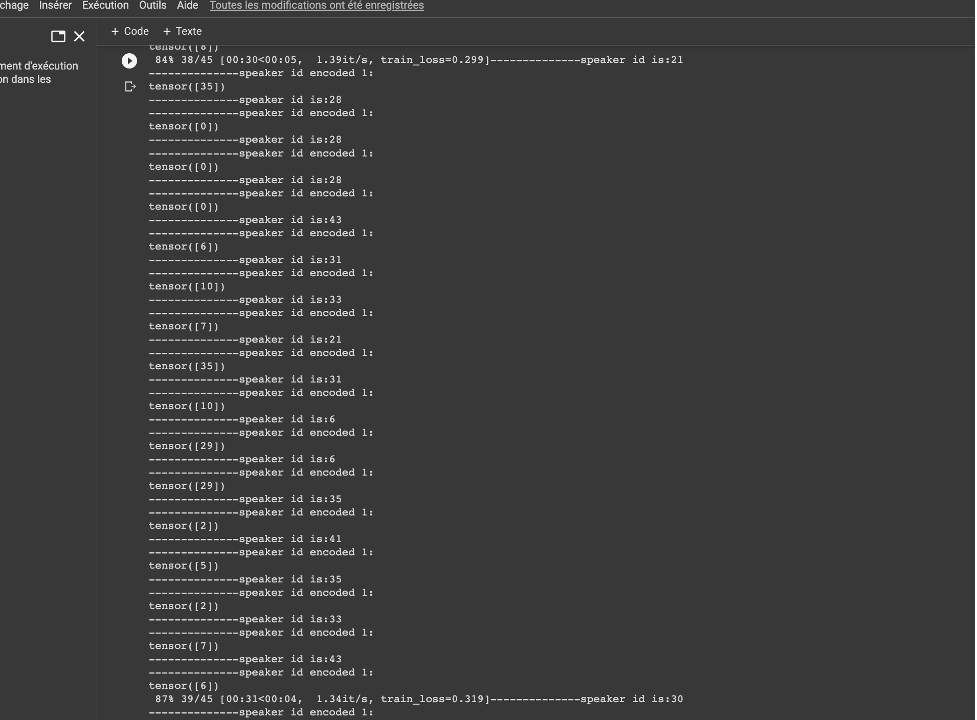
\includegraphics[width=1\textwidth]{3chap24}
	\caption{Logs de l’entrainement variation de la function loss}
	\label{fig:3chap24}
\end{figure}

\begin{figure}[h]
	\centering
	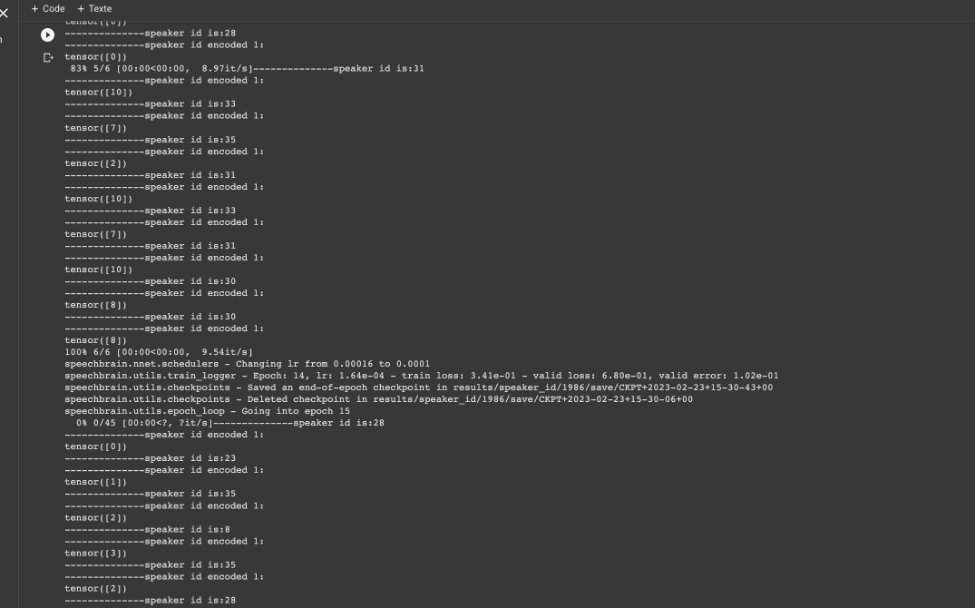
\includegraphics[width=1\textwidth]{3chap25}
	\caption{Logs de l’entrainement, passage de l’Epoch 14 à l’Epoch 15}
	\label{fig:3chap25}
\end{figure}

Voyons quels fichiers/dossiers sont générés dans le output\_folder spécifié :
\begin{itemize}
    \item \textbf{train\_log.txt} : contient les statistiques (par exemple, train\_loss, valid\_loss) calculées à chaque époque.
    \item \textbf{log.txt} : est un enregistreur plus détaillé contenant les horodatages pour chaque opération de base.
    \item \textbf{env.log} : affiche toutes les dépendances utilisées avec leur version correspondante (utile pour la réplicabilité).
    \item \textbf{train.py, hyperparams.yaml }: sont une copie du fichier d'expérience avec les hyperparamètres correspondants 
    \item \textbf{save} : est l'endroit où nous stockons le modèle généré.

\end{itemize}

Dans le dossier de sauvegarde, on a des sous-dossiers contenant les points de contrôle enregistrés lors de l'entraînement (au format CKPT+données+heure). Typiquement, on y trouve ici deux points de contrôle : le meilleur (c'est-à-dire le plus ancien) et dernier (c'est-à-dire le plus récent). 
\begin{figure}[h]
	\centering
	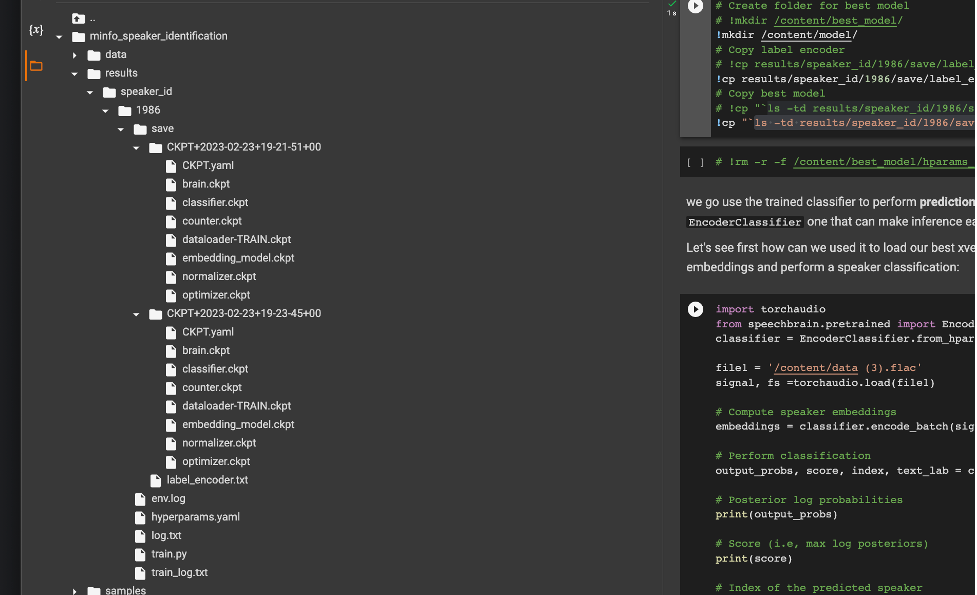
\includegraphics[width=1\textwidth]{3chap26}
	\caption{Les deux models }
	\label{fig:3chap26}
\end{figure}

À l'intérieur de chaque point de contrôle, nous stockons toutes les informations nécessaires pour reprendre l’entrainement (par exemple, les modèles, les optimiseurs, les planificateurs, le compteur d'époques, etc.). Les paramètres des modèles d'intégration sont rapportés dans le fichier embedding\_model.ckpt, tandis que ceux du classifieur sont dans classifier.ckpt. C'est juste un format binaire lisible avec torch.load.
Le dossier de sauvegarde contient également l'encodeur d'étiquette (label\_encoder.txt), qui mappe chaque entrée d'id de locuteur à leurs index correspondants.
A la fin de l’entrainement, l'erreur de validation doit passer à zéro (ou très proche de zéro).

\section{Inférence}
À ce stade, nous pouvons utiliser notre meilleur model pour effectuer des prédictions sur de nouvelles données. Speechbrain dispose de la classe EncoderClassifier qui facilite l'inférence. La classe peut également être utilisée pour extraire certains plongements à la sortie de l'encodeur.
Voyons d'abord comment pouvons-nous l'utiliser pour charger notre meilleur modèle xvector   pour  effectuer une classification des locuteurs :

\begin{figure}[h]
	\centering
	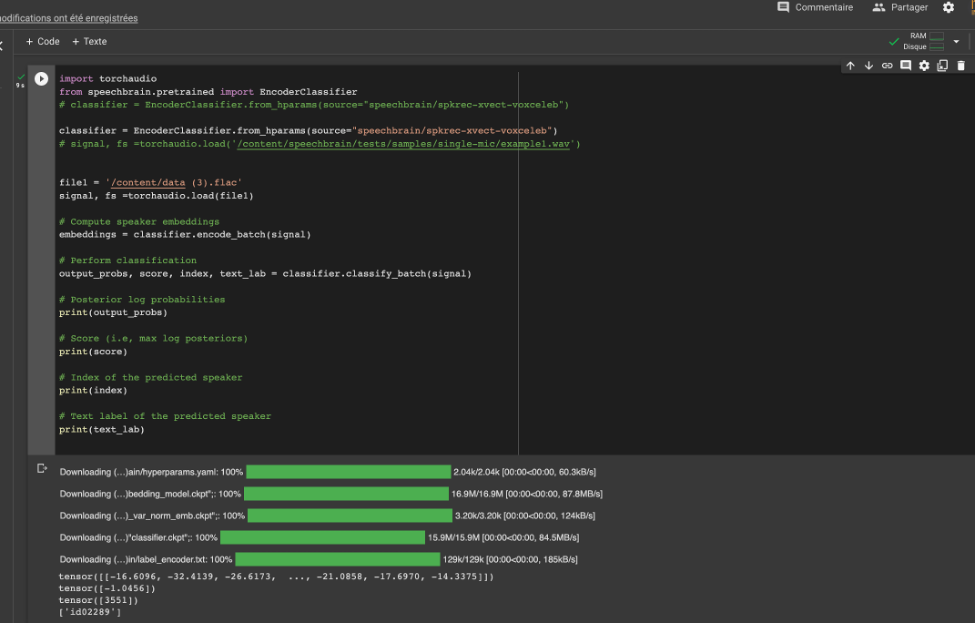
\includegraphics[width=1\textwidth]{3chap27}
	\caption{Préparation du model  }
	\label{fig:3chap27}
\end{figure}

Mais comment cela fonctionne-t-il avec notre model que nous avons formé auparavant ?

\begin{figure}[h]
	\centering
	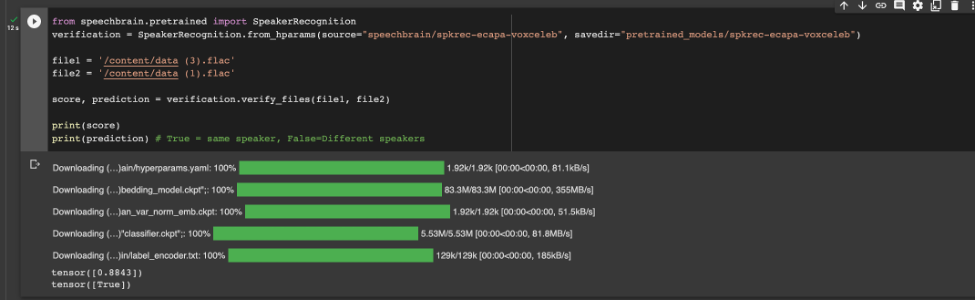
\includegraphics[width=1\textwidth]{3chap28}
	\caption{Inférence sur le modèle pour l'authentification }
	\label{fig:3chap28}
\end{figure}

Exemple d’inférence pour l’authentication. le résultat est contenue dans la variable prédiction (voir figure \ref{fig:3chap28})(True = le locuteur est bien celui dont il s’agit, False=Le locuteur n’est pas celui qu’il prétend). 


\begin{figure}[h]
	\centering
	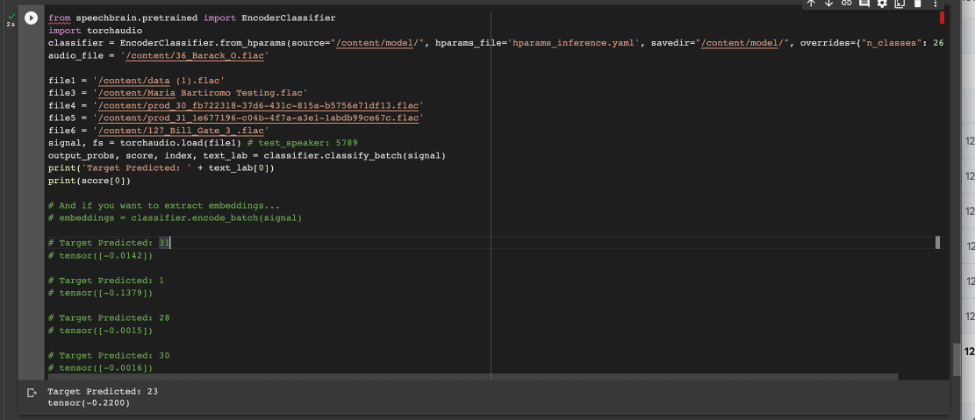
\includegraphics[width=1\textwidth]{3chap29}
	\caption{Inférence sur le modèle pour l'identification }
	\label{fig:3chap29}
\end{figure}
Ici nous avons effectué l’inférence pour l’identification de locuteur ce qui nous a retourné le locuteur avec l’ID 23 (voir figure \ref{fig:3chap29}).

\section{Le développement des Apis}
A cette étape, nous pouvons exporter notre model vers Cloud Storage afin de pouvoir l’utiliser sur notre backend Django.
Le code se presnte comme suit :



\begin{itemize}
    \item UpdateModel cette classe permet de recupere le dernier modeldepui Cloud Storage pour l’utilisation a des fin de reconnaissance. \\\textbf{Requête : GET} \\\textbf{Route : https://api.dev.minfo.com/api/speaker/updatemodel }
	\lstinputlisting[language=Python,  firstline=155, lastline=186]{views.py}

	
    \item \textbf{IdentifySpeaker}: Cette classe permet d’identifier le locuteur. \\\textbf{Requête : POST} \\\textbf{Route : https://api.dev.minfo.com/api/speaker/id}
	\lstinputlisting[language=Python,  firstline=72, lastline=151]{views.py}

    \item \textbf{MatchVoices}: Elle permet d’authentifier un locuteur. \\\textbf{Requête : POST} \\\textbf{Route : https://api.dev.minfo.com/api/speaker/match}
	\lstinputlisting[language=Python,  firstline=12, lastline=46]{views.py}

\end{itemize}

% \begin{lstlisting}[language=Python, caption=Python example]
% 	import numpy as np
		
% 	def incmatrix(genl1,genl2):
% 		m = len(genl1)
% 		n = len(genl2)
% 		M = None #to become the incidence matrix
% 		VT = np.zeros((n*m,1), int)  #dummy variable
		
% 		#compute the bitwise xor matrix
% 		M1 = bitxormatrix(genl1)
% 		M2 = np.triu(bitxormatrix(genl2),1) 
	
% 		for i in range(m-1):
% 			for j in range(i+1, m):
% 				[r,c] = np.where(M2 == M1[i,j])
% 				for k in range(len(r)):
% 					VT[(i)*n + r[k]] = 1;
% 					VT[(i)*n + c[k]] = 1;
% 					VT[(j)*n + r[k]] = 1;
% 					VT[(j)*n + c[k]] = 1;
					
% 					if M is None:
% 						M = np.copy(VT)
% 					else:
% 						M = np.concatenate((M, VT), 1)
					
% 					VT = np.zeros((n*m,1), int)
		
% 		return M
% 	\end{lstlisting}

\addcontentsline{toc}{section}{Conclusion}
\section*{Conclusion}
Dans cette partie, nous avons montré comment créer un model TDNN pour l’authentication et l’identification des locuteurs. Le système proposé contient tous les ingrédients de base pour développer un système de pointe (c'est-à-dire, l'augmentation de données, l'extraction de caractéristiques, l'encodage, la mise en pool statistique, le classificateur, etc.).
Dans le prochain chapitre nous présenterons les résultats obtenus après notre implémentation. 


 \chapter{Résultats et discussions}\label{chap:4}
 \addcontentsline{toc}{section}{Introduction}
\section*{Introduction}
Dans ce chapitre, nous présentons les différentes fonctionnalités de notre système.   Les résultats obtenus sont assez satisfaisants. Ces résultats encourageants montrent des possibilités d'adoption de la reconnaissance de locuteur dans divers domaines, tels que la sécurité biométrique pour l'identification de personnes, la surveillance des appels téléphoniques, les centres d'appels et les interactions vocales dans les voitures connectées. Dans ce chapitre, nous repréciserons le cadre d’étude de notre système, ainsi que lesdits résultats, obtenus à l’issue de l’implémentation. 

\section{Présentation du cadre d’étude}
Le présent système mis sur pieds a pour but la reconnaissance de locuteur.
La reconnaissance de locuteur est une application de l'intelligence artificielle (IA) qui vise à identifier et à authentifier une personne en fonction de sa voix. 
Cette technologie peut être utilisée dans différents contextes tels que la sécurité, l'assistance vocale, la gestion de la relation client, etc. 
l’IA pourra être déployée et mise à la disposition des services de la criminologie pour servir lors des enquêtes judiciaires pour identifier des individus. 
Elle pourra également servir à sécuriser les systèmes en implémentant un MFA (Multi-Factor Authentication) afin d’accroitre la sécurité des systèmes.


\section{Résultats obtenus}
Nous rappelons que la génération de nos modèles, à partir des données d’apprentissage a été possible grâce au service cloud de Google Colaboratory . Celui-ci est un outil intuitif donnant accès à des ressources informatiques permettant de travailler sur des projets en science des données. Par la suite ces modèles ont été sauvegardé sur Cloud Storage afin d’alimenter notre application Django qui offrira les APIs pour les opérations d’identification et d’authentification.
L'utilisation de l'IA pour la reconnaissance de locuteur a connu une avancée significative au cours des dernières années grâce à l'amélioration des algorithmes d'apprentissage automatique et de traitement du signal vocal. Les résultats obtenus sont encourageants et permettent d'identifier un locuteur avec une précision élevée.
Les tests réalisés sur des enregistrements de voix ont montré que l'IA est capable de reconnaître un locuteur avec une précision pouvant varier en fonction de la qualité de l'enregistrement, du bruit ambiant et de la durée de la parole. 

\subsection{liste des locuteurs}
La figure suivante présente la liste des locuteurs. Dans notre architecture, nous les avons appelé POI (Person Of Interest). 

\begin{figure}[h]
	\centering
	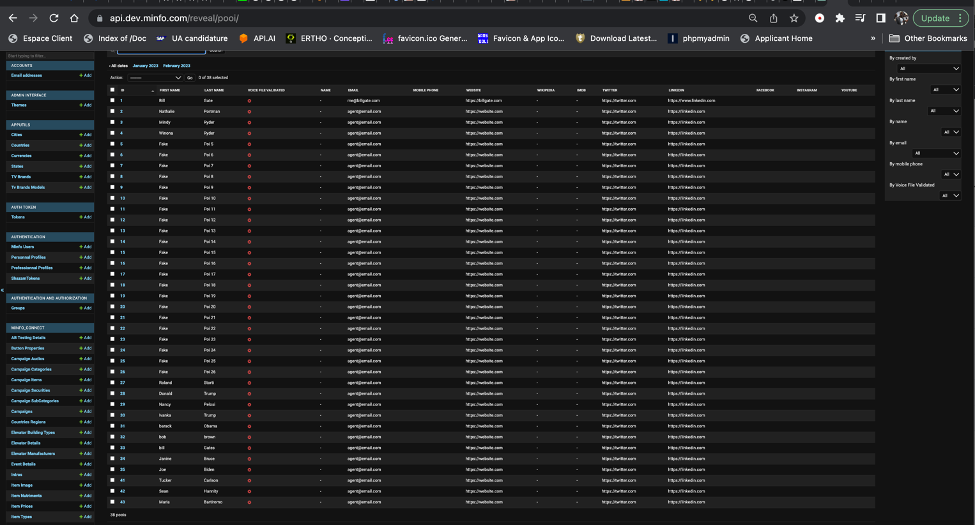
\includegraphics[width=1\textwidth]{4chap1}
	\caption{Liste des POI}
	\label{fig:4chap1}
\end{figure}
A partir de cette page nous pouvons facilement étendre la liste, ajouter des empreintes vocales pour les différents POIs.

\subsection{mise à jour du model}
Après l’entrainement sur Google Colab, le model est exporté vers Cloud Storage pour usage ultérieure.

\begin{figure}[h]
	\centering
	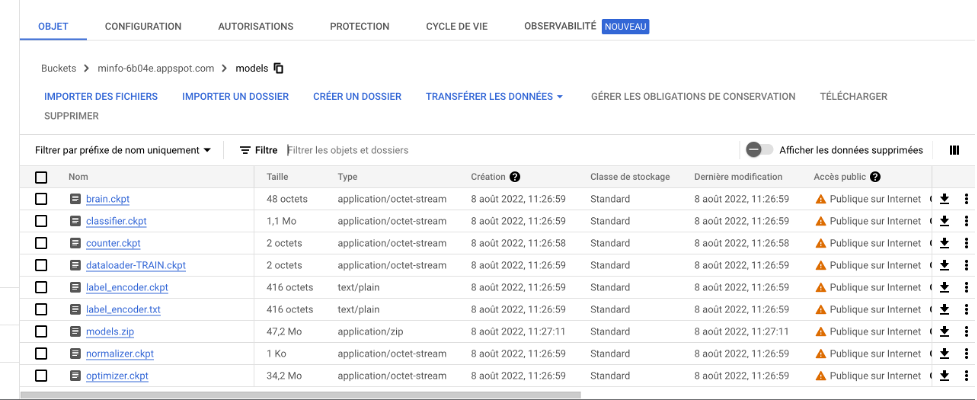
\includegraphics[width=1\textwidth]{4chap2}
	\caption{Meilleure modèle sauvegardé sur Cloud Storage}
	\label{fig:4chap2}
\end{figure}
Afin de récupérer ce model et l’utiliser en production dans notre projet Django, nous appelons la route  \textbf{api/speaker/updatemodel}

\begin{figure}[h]
	\centering
	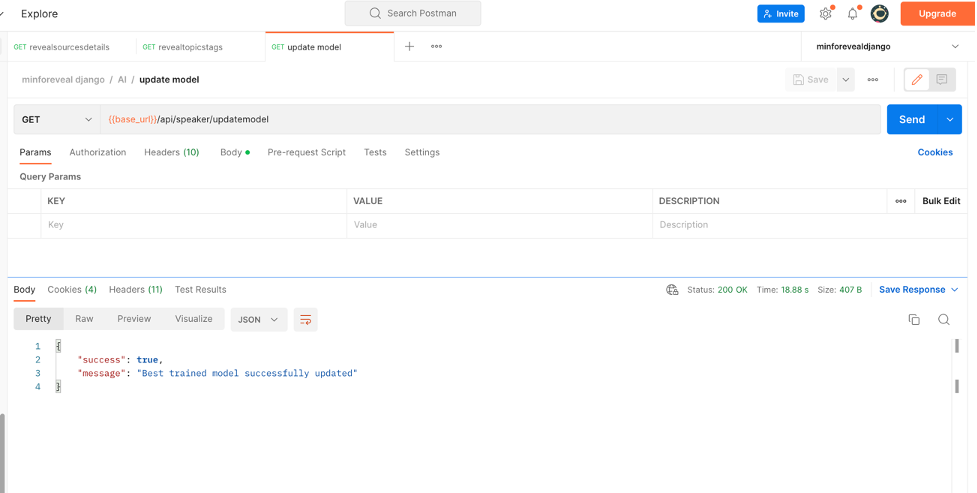
\includegraphics[width=1\textwidth]{4chap3}
	\caption{récupération du meilleur modèle}
	\label{fig:4chap3}
\end{figure}

\subsection{Identification de locuteur}
L’identification répond à la question : « Qui est cette personne ? ». Elle consiste à vérifier dans notre base de données à qui correspond une empreinte vocale.  

\begin{figure}[h]
	\centering
	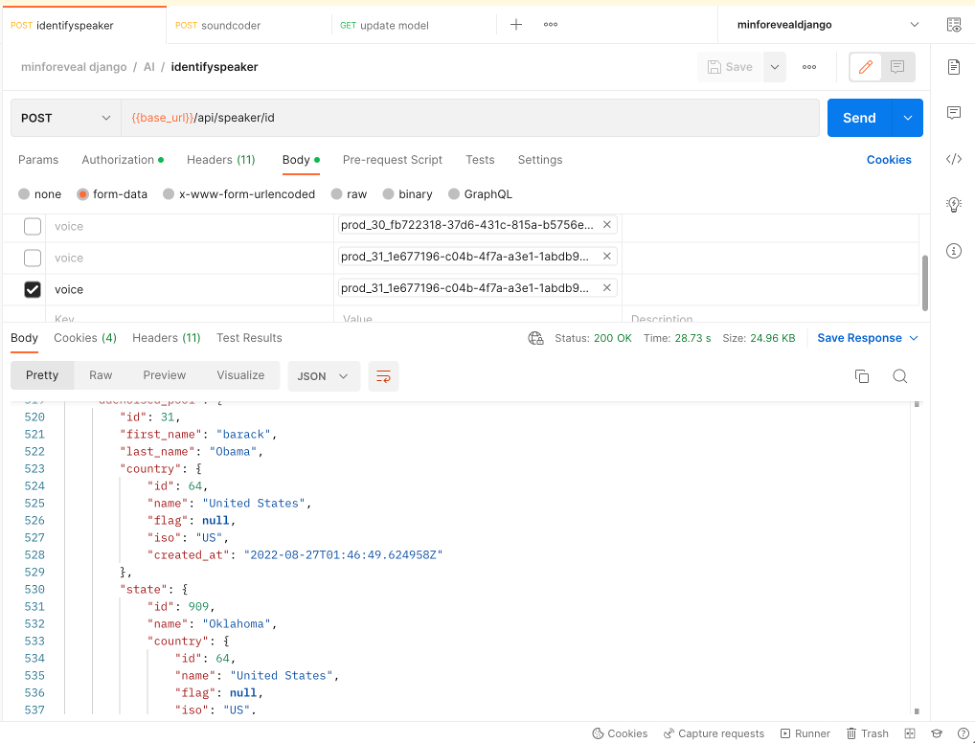
\includegraphics[width=1\textwidth]{4chap4}
	\caption{Identification de locuteur}
	\label{fig:4chap4}
\end{figure}
\textbf{Route:  /api/speaker/id}
\\\textbf{Requête : POST}
\\\textbf{Paramètre : voice(le fichier vocal)}
\\\textbf{Le locuteur doit être dans la liste des POI.}

\subsection{authentification de locuteur}
L’authentification permet de répondre à la question : « Le locuteur est-il vraiment celui qu’il prétend être ? ». Pour cet API on n’a pas besoin d’avoir les empreintes vocales du locuteur. Ainsi la plateforme qui intègre l’API peut conserver ses empreintes sur ses serveurs privés cela resoud en même temps les problématiques de privilèges d’accès aux données, de sécurités et de confidentialité.
\\\textbf{route  /api/speaker/match}
\\\textbf{Requête : POST}
\\\textbf{Paramètre : voice1 et voice2(le fichier vocal empreinte et le fichier vocale enregistré à l’authentification)}
\\\textbf{Le locuteur n’a pas besoin d’être enregistré dans la base des POI.}

\begin{figure}[h]
	\centering
	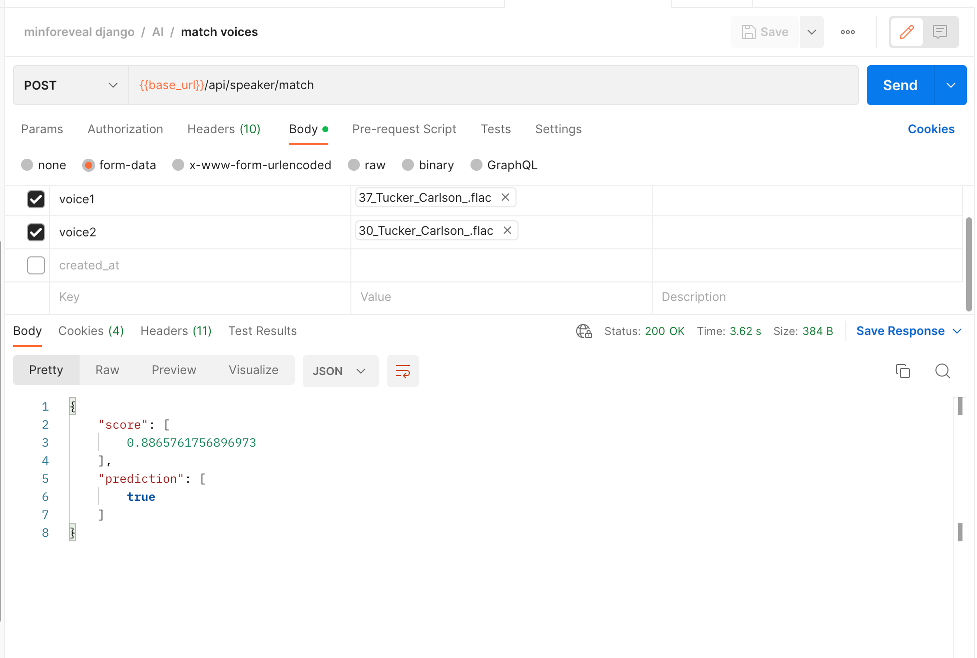
\includegraphics[width=1\textwidth]{4chap5}
	\caption{Identification de locuteur}
	\label{fig:4chap5}
\end{figure}

\paragraph{}La prédiction représente le résultat de l’authentication :

\begin{itemize}
    \item True signifie que l’utilisateur est bien celui qu’il prétend être
    \item False signifie que l’utilisateur n’est pas le bon, c’est-à-dire que la voix ne correspond pas à l’empreinte vocale.
\end{itemize}

\subsection{Analytic des connexions}
Nous avons mise en place un service d’analytique pour le suivi et l’utilisation du système. Il enregistre la date, le fichier vocal et le résultat du scan. 


\begin{figure}[h]
	\centering
	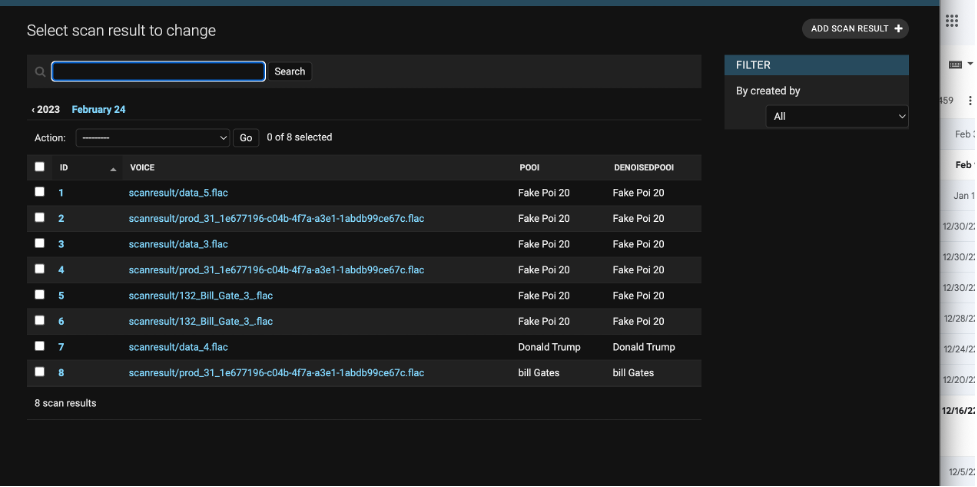
\includegraphics[width=1\textwidth]{4chap6}
	\caption{Identification de locuteur}
	\label{fig:4chap6}
\end{figure}

\section{avantage de notre architecture}
Le TDNN (Time Delay Neural Network) est l’architecture de réseau de neurones artificiels qui a été utilisée dans. Le cas de notre étude pour la reconnaissance de locuteur. Concernant ses avantages, nous pouvons citer :
\begin{itemize}
    \item Le TDNN est relativement rapide à entraîner et à utiliser une fois qu'il a été entraîné.
    \item Les TDNN peuvent prendre en compte les caractéristiques temporelles des signaux acoustiques. En effet, les TDNN sont capables de prendre en compte les données d'entrée passées et présentes, ce qui est important pour la reconnaissance de locuteur.
    \item Les TDNN peuvent être utilisés pour extraire des caractéristiques discriminantes des signaux acoustiques. Les TDNN peuvent apprendre des caractéristiques complexes des signaux acoustiques, ce qui est important pour la reconnaissance de locuteur.
    \item Les TDNN peuvent être entraînés sur de grandes quantités de données. Les TDNN sont capables d'apprendre à partir de grandes quantités de données, ce qui est important pour la reconnaissance de locuteur.
\end{itemize}

\section{Les limites de notre architecture}
Il convient de noter que les inconvénients du TDNN pour la reconnaissance de locuteurs peuvent varier en fonction du contexte d'utilisation et des caractéristiques des données de parole utilisées pour l'entraînement et le test.
Les TDNN peuvent être sensibles aux variations de conditions d'enregistrement. Les TDNN peuvent être affectés par des facteurs tels que le bruit de fond, la qualité de l'enregistrement, la distance entre le locuteur et le microphone, etc.
Les TDNN peuvent nécessiter une grande quantité de données d'entraînement. Pour obtenir des performances de reconnaissance de locuteur élevées, il peut être nécessaire de disposer d'une grande quantité de données d'entraînement.
Les TDNN peuvent nécessiter une puissance de calcul importante. L'entraînement et l'utilisation de TDNN peut être coûteux en termes de puissance de calcul, surtout lorsqu'il s'agit de grandes quantités de données.

\addcontentsline{toc}{section}{Conclusion}
\section*{Conclusion}
Dans ce chapitre, nous avons présenté les résultats obtenus à travers quelques figures présentants l’utilisation de nos different APIs.
Dans le cas où l'IA est bien entraînée avec des données de haute qualité et utilisée dans un contexte approprié, elle peut fournir une reconnaissance de locuteur précise et fiable. Cela peut être utile dans diverses applications, telles que la sécurité de l'authentification vocale, l'analyse de la parole pour la recherche et la reconnaissance de locuteur dans les applications de communication.
Cependant, l'utilisation d'une IA pour la reconnaissance de locuteur peut également soulever des préoccupations en matière de vie privée et de sécurité. Si les données vocales utilisées pour entraîner l'IA sont mal protégées, elles peuvent être utilisées pour identifier les utilisateurs sans leur consentement, ou même être utilisées à des fins malveillantes. Il est donc important de prendre des mesures pour protéger la vie privée des utilisateurs et de veiller à ce que l'utilisation de l'IA pour la reconnaissance de locuteur soit justifiée et éthique. C’est pour ça que notre implémentation de l’authentification renécessite pas une sauvegarde par notre système des empreinte vocaux. 
En résumé, l'utilisation d'une IA pour la reconnaissance de locuteur peut être utile dans certains contextes, mais elle nécessite une attention particulière pour garantir la précision, la fiabilité et la protection de la vie privée des utilisateurs.


% \include{perspectives}
%%conclusion
\conclusion
%Bla bla bla \cite{ehrig2006graph}
\paragraph{}La mise en place d'une IA pour la reconnaissance de locuteur est un domaine en constante évolution qui présente des opportunités importantes pour de nombreuses applications dans diverses industries. Les avancées dans les domaines de l'apprentissage automatique, du traitement du signal et de la reconnaissance de la parole ont permis de développer des systèmes de reconnaissance de locuteur de plus en plus précis et efficaces.	
\paragraph{}Dans le domaine de la sécurité, l'IA peut être utilisée pour identifier des individus spécifiques en fonction de leur voix, ce qui peut aider à identifier des criminels ou des suspects dans une enquête. Dans les centres d'appels, l'IA peut aider à identifier automatiquement les appelants enregistrés, ce qui peut aider à accélérer le processus d'identification et améliorer l'efficacité du centre d'appels.
\paragraph{}Dans le domaine de l'assistance aux personnes âgées ou atteintes de troubles cognitifs, l'IA peut aider à identifier les membres de la famille ou les amis d'un patient par leur voix, ce qui peut aider à améliorer leur qualité de vie et leur sécurité.
\paragraph{}Cependant, la mise en place de ces systèmes soulève également des questions éthiques et de confidentialité. Il est important de garantir que les données des utilisateurs soient traitées de manière éthique et sécurisée, conformément aux lois et réglementations applicables.
\paragraph{}Pour l'avenir, il est possible que les systèmes de reconnaissance de locuteur soient intégrés dans une gamme encore plus large de dispositifs et de technologies, ce qui permettrait une interaction plus intuitive entre les humains et les machines. Par exemple, les voitures autonomes pourraient utiliser la reconnaissance vocale pour identifier les conducteurs et les passagers, ou les appareils médicaux pourraient être configurés pour reconnaître la voix d'un patient afin de personnaliser les soins.
\paragraph{}En fin de compte, la mise en place d'une IA pour la reconnaissance de locuteur présente à la fois des opportunités et des défis, et il est important d'évaluer soigneusement les avantages et les risques potentiels avant de l'utiliser dans une application spécifique.
\paragraph{}En perspectives, nous comptons ajouter d’autres fonctionnalités, poursuivre nos travaux de recherche afin de perfectionner au mieux le model pour aboutir à une solution beaucoup plus optimale. Il s’agira aussi de le mettre en place avec d’autres méthodes et algorithme de Deep Learning pour comparer les performances. 

% 
\lhead[]{} \rhead[]{} \chead[]{}

%%biblio
\addcontentsline{toc}{chapter}{Bibliographie}
\bibliographystyle{abbrv}
\bibliography{biblio}


%\chapter*{Annexe}\addcontentsline{toc}{chapter}{Annexe}\label{annexe1}

\subsection*{Étapes clés du déroulement de l'attaque}


Nous allons exploiter quelques failles de ce réseau pour effectuer une attaque man in the middle (MITM).\\

Au début, notre machine Windows peut atteindre normalement le routeur R4.
\begin{figure}[H]
    \centering
    \includegraphics[scale=0.8]{images/ping_b4_1}
    \caption{Ping vers le routeur R4 avec succès}
    \label{fig:ping_b4_1}
\end{figure}
Quand on essaie de tracer le chemin vers R4, on constate que la machine passe par le routeur R1 légitime du lien pour atteindre R4
\begin{figure}[H]
    \centering
    \includegraphics{images/tracert_b4_1}
    \caption{Traces du chemin vers R4}
    \label{fig:tracert_b41}
\end{figure}
L'attaquant sur le lien peut alors passer a l'attaque.
Pour effectuer l'attaque MITM on utilisera l'outil fake\_router6, un utilitaire du package d'outils \textbf{the hacker choice}.
Ainsi sur la machine d'attaque, on active en un premier lieu le forwarding pour être transparent et ne pas bloquer le transit des paquets.
\begin{figure}[H]
    \centering
    \includegraphics{images/attk/fwrd_activation}
    \caption{Activation du forwarding des paquets.}
    \label{fig:activ_fwrd}
\end{figure}
Aussi on lance wireshark pour observer le trafic des paquets sur notre interface dans le réseau.\\
-------\\
Puisque tout est prêt nous allons lancer l'attaque.

\begin{figure}[H]
    \centering
    \includegraphics[scale=0.8]{images/attk/lancement_attk_1}
    \caption{Initialisation de l'attaque}
    \label{fig:attk_init_1}
\end{figure}

L'attaque est en cours et l'attaquant s'annonce comme le routeur par défaut du lien
nous allons maintenant vérifier la table des routes de notre machine windows.
\begin{figure}[H]
    \centering
    \includegraphics{images/attk/tableRoutes_windows}
    \caption{Table des routes de la machine victime}
    \label{fig:win_route_table}
\end{figure}
On constate que l'attaquant s'est insère comme passerelle de la victime.
pour confirmer cela reprenons un tracert vers le routeur r4
\begin{figure}[H]
    \centering
    \includegraphics{images/attk/tracert_b4_2}
    \caption{Chemin vers b4 pendant l'attaque.}
    \label{fig:tracert_b42}
\end{figure}
On peut voir clairement que la victime passe par l'attaquant pour atteindre le routeur.\\

A présent nous allons essayer de capturer une information envoyée par la victime.
Pour cela la victime fait un telnet sur le router R4 pour s'y connecter avec les paramètres suivants:\\
password1:\textbf{cisco}\\
password2:\textbf{class}
\begin{figure}[H]
    \centering
    \includegraphics{images/attk/telnet_r4}
    \caption{Connexion telnet au routeur.}
    \label{fig:telnetr4}
\end{figure}

Une fois la connexion réussie, nous allons voir avec wireshark les paquets de connexion et y retrouver les paramètres de connexion.
\begin{figure}[H]
    \centering
    \includegraphics[width=1.0\textwidth]{images/attk/c}
    \includegraphics[width=1.0\textwidth]{images/attk/i}
    \includegraphics[width=1.0\textwidth]{images/attk/s}
    \includegraphics[width=1.0\textwidth]{images/attk/c2}
    \includegraphics[width=1.0\textwidth]{images/attk/o}   
    \caption{Premier paramètre de connexion au routeur R4: \textbf{c-i-s-c-o}}
    \label{fig:param_conn_r4}
\end{figure}
\begin{figure}[H]
    \centering
    \includegraphics[width=1.0\textwidth]{images/attk/param2_c}
    \includegraphics[width=1.0\textwidth]{images/attk/param2_l}
    \includegraphics[width=1.0\textwidth]{images/attk/param2_a}
    \includegraphics[width=1.0\textwidth]{images/attk/param2_s1}
    \includegraphics[width=1.0\textwidth]{images/attk/param2_s2}
    \caption{Second paramètre de connexion au routeur R4: \textbf{c-l-a-s-s}}
    \label{fig:param_conn2}
\end{figure}
Les paramètres on été retrouves donc l'attaque a été un succès!

%\subsection*{Mitigations}
%Pour sécuriser ce réseau afin d'éviter ce genre d'attaque, deux mesures de sécurité peuvent être configurées.
%\begin{itemize}
%    \item le SEND
%    \item le RaGuard
%\end{itemize}



\newpage
\tableofcontents

\end{document}          
         
